\chapter{The CMS experiment at the LHC}\label{ch:cms}

\section{Introduction}\label{sec:cms_intro}
\noindent Located in the Swiss-French border, the European Council for Nuclear Research (CERN) is the largest scientific organization leading the particle physics research. About 13000 people in a broad range of fields including users, students, scientists, engineers among others, contribute to the data taking and analysis, with the goal of unveiling the secrets of the nature and revealing the fundamental structure of the universe. CERN is also the home of the Large Hadron Collider (LHC), the largest circular particle accelerator around the world, where protons (or heavy ions) traveling close to the speed of light, are made to collide. These collisions open a window to investigate how particles (and their constituents if they are composite) interact with each other, providing clues about the laws of the nature. This chapter present an overview of the LHC structure and operation. A detaled description of the CMS detector is offered, given that the data used in this thesis have been taken with this detector.     

\section{The LHC}

\noindent With 27 km of circunference, the LHC is currently the largest and most powerful accelerator in the world. It is installed in the same tunnel where the large Electron-Positron (LEP) collider was located, taking advantage of the existing infraestructure. The LHC is also the larger accelerator in the CERN's accelerator complex and is assisted by several successive accelerating stages before the particles are injected into the LHC ring where they reach their maximum eneregy (see figure \ref{fig:cern}).

\begin{figure}[!h]
  \centering
  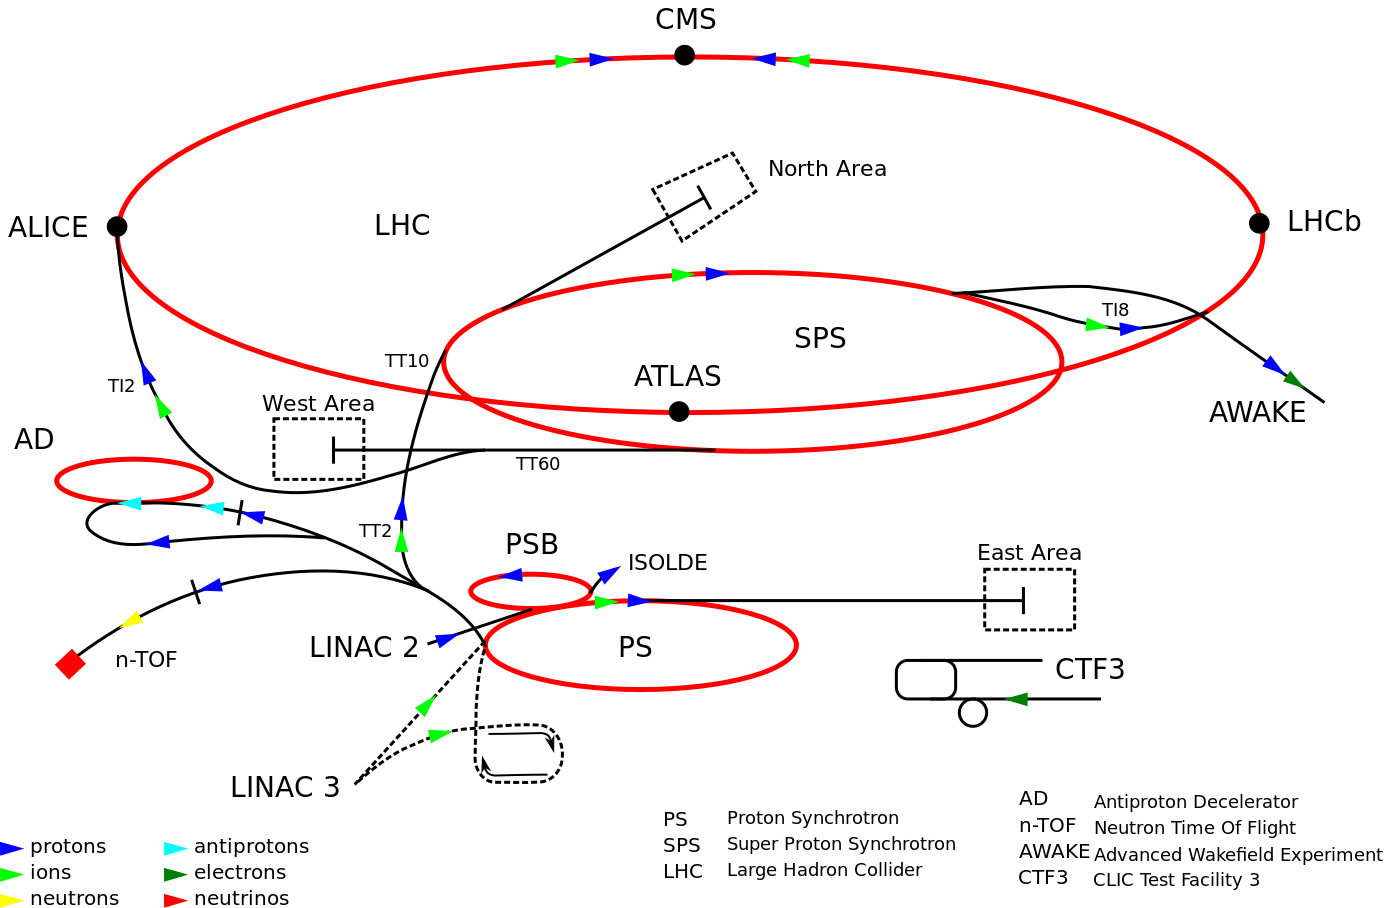
\includegraphics[width=0.7\textwidth]{cern_ac}
  \caption[CERN accelerator complex]{CERN accelerator complex. Blue arrows show the path followed by protons along the acceleration process \cite{cern}.}\label{fig:cern}
\end{figure}

\noindent LHC run in three modes depending on the particles being accelerated

\begin{itemize}
\item Proton-Proton collisions (pp) for multiple physics experiments.
\item Lead-Lead collisions (Pb-Pb) for heavy ion experiments. 
\item Proton-Lead collisions (p-Pb) for quark-gluon plasma experiments.
\end{itemize}

\begin{figure}[!h]
\centering
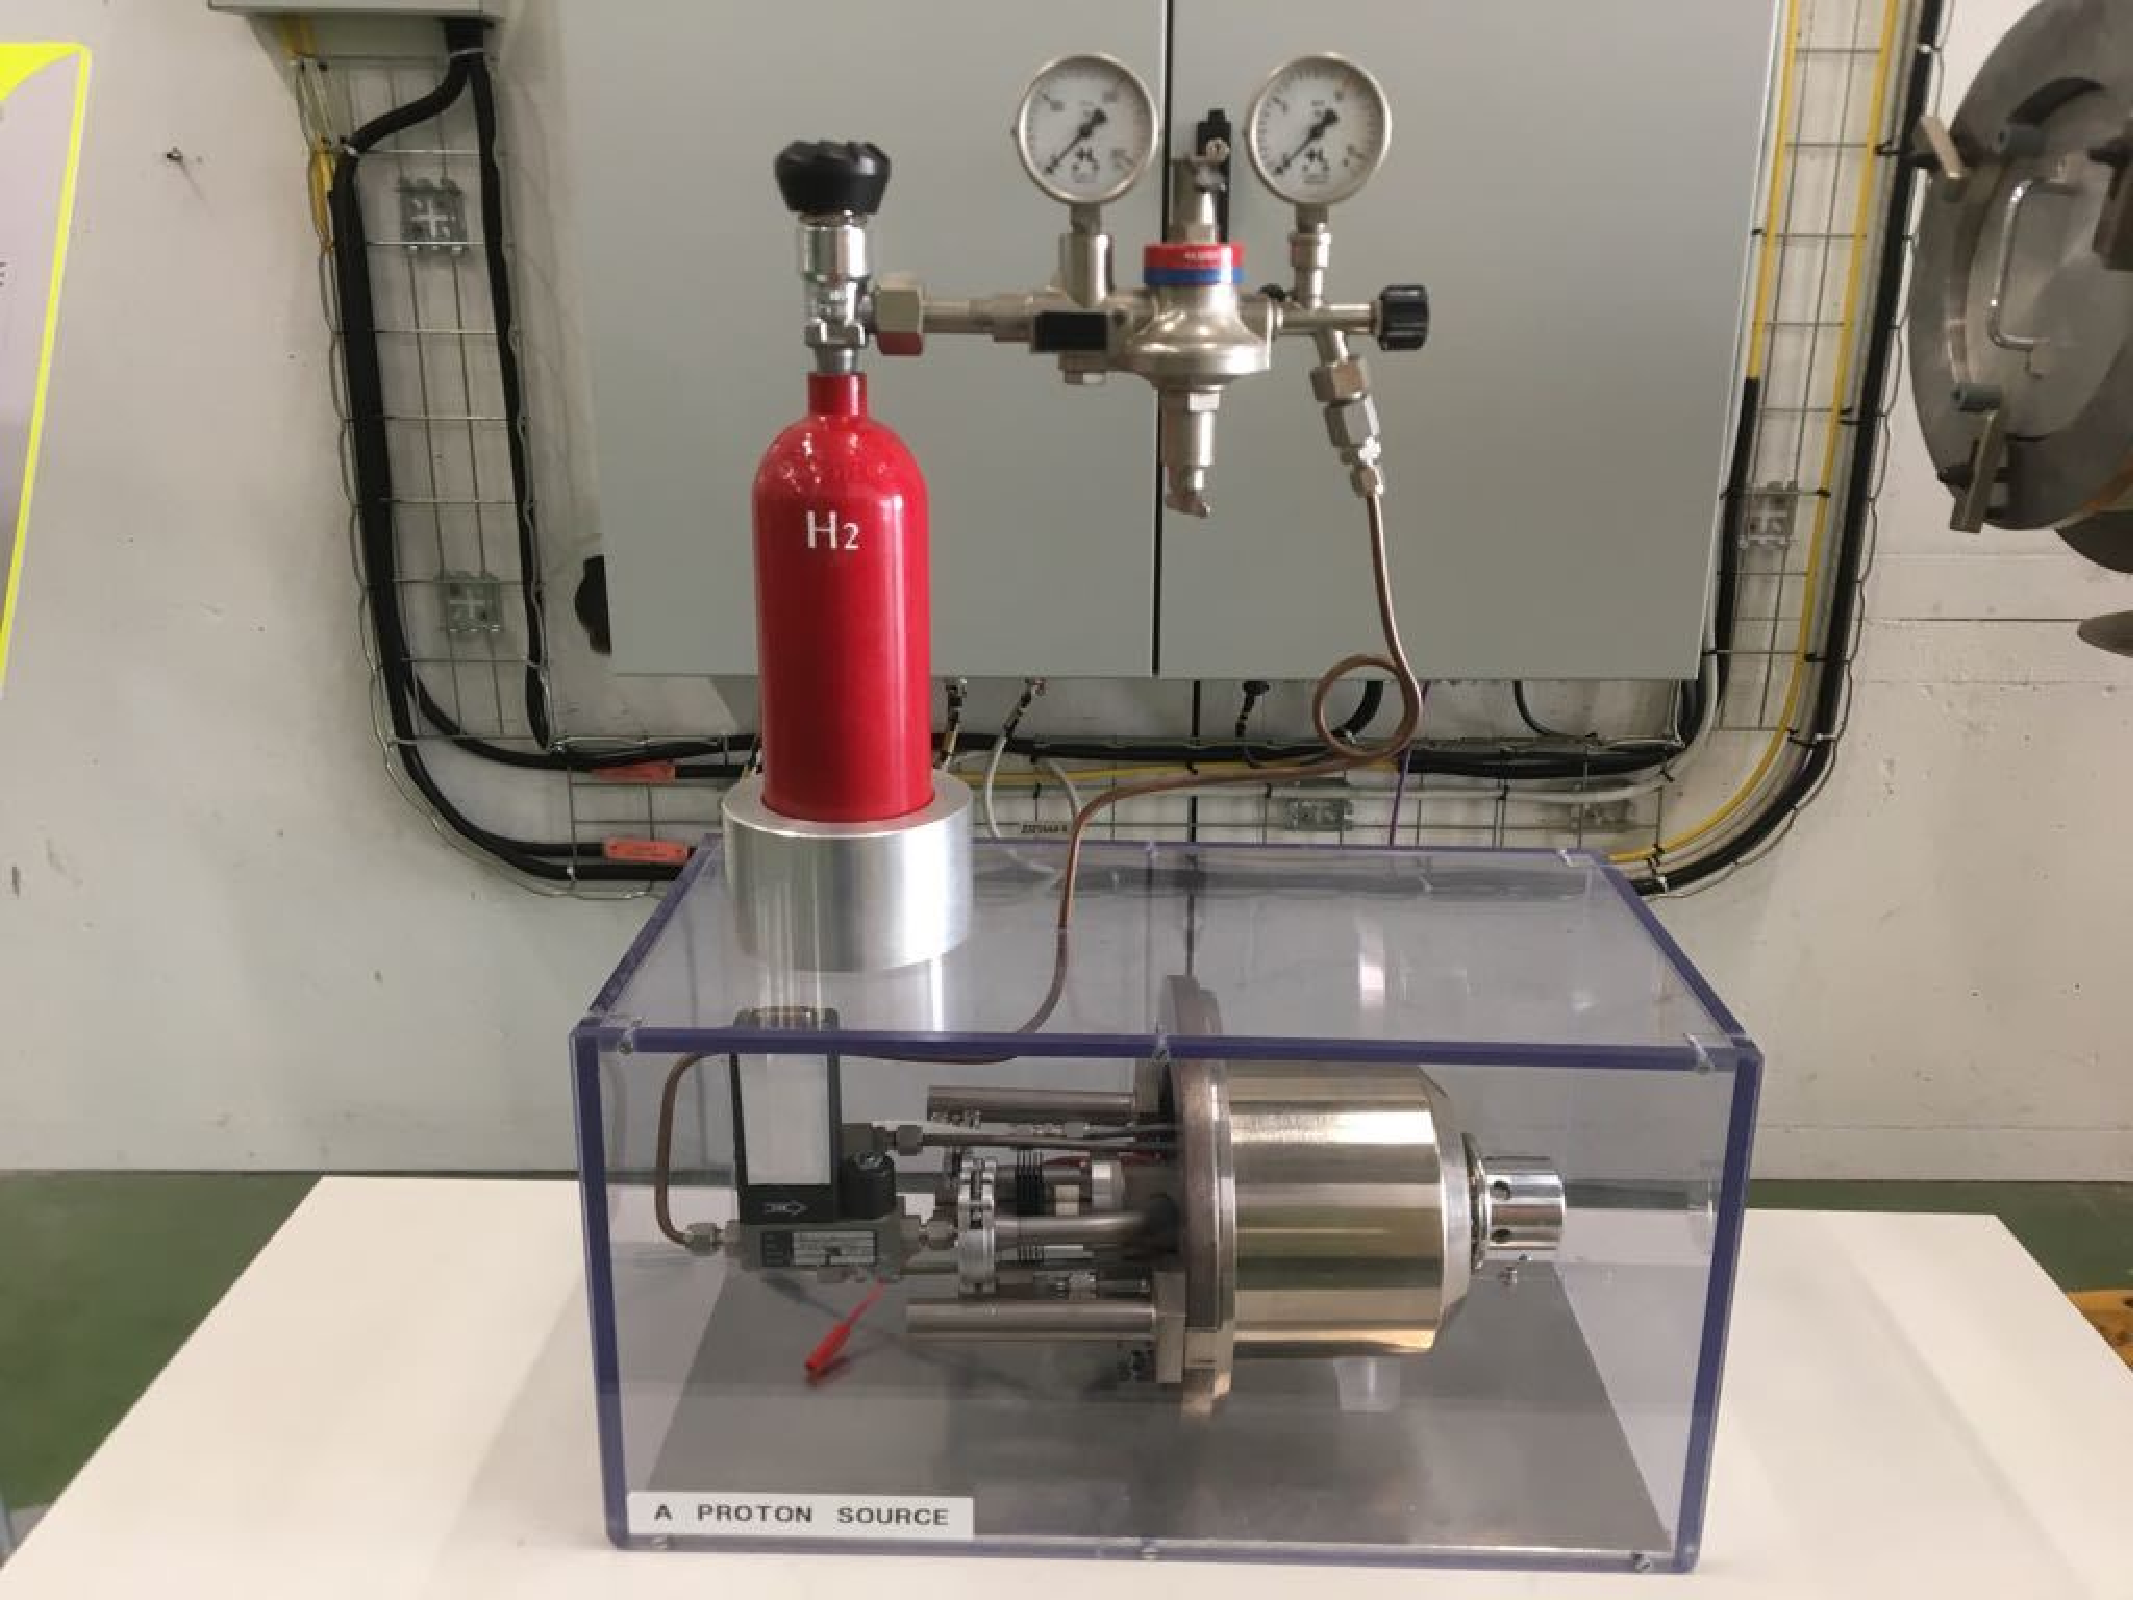
\includegraphics[width=4.5cm,height=3.3cm]{hbottle}
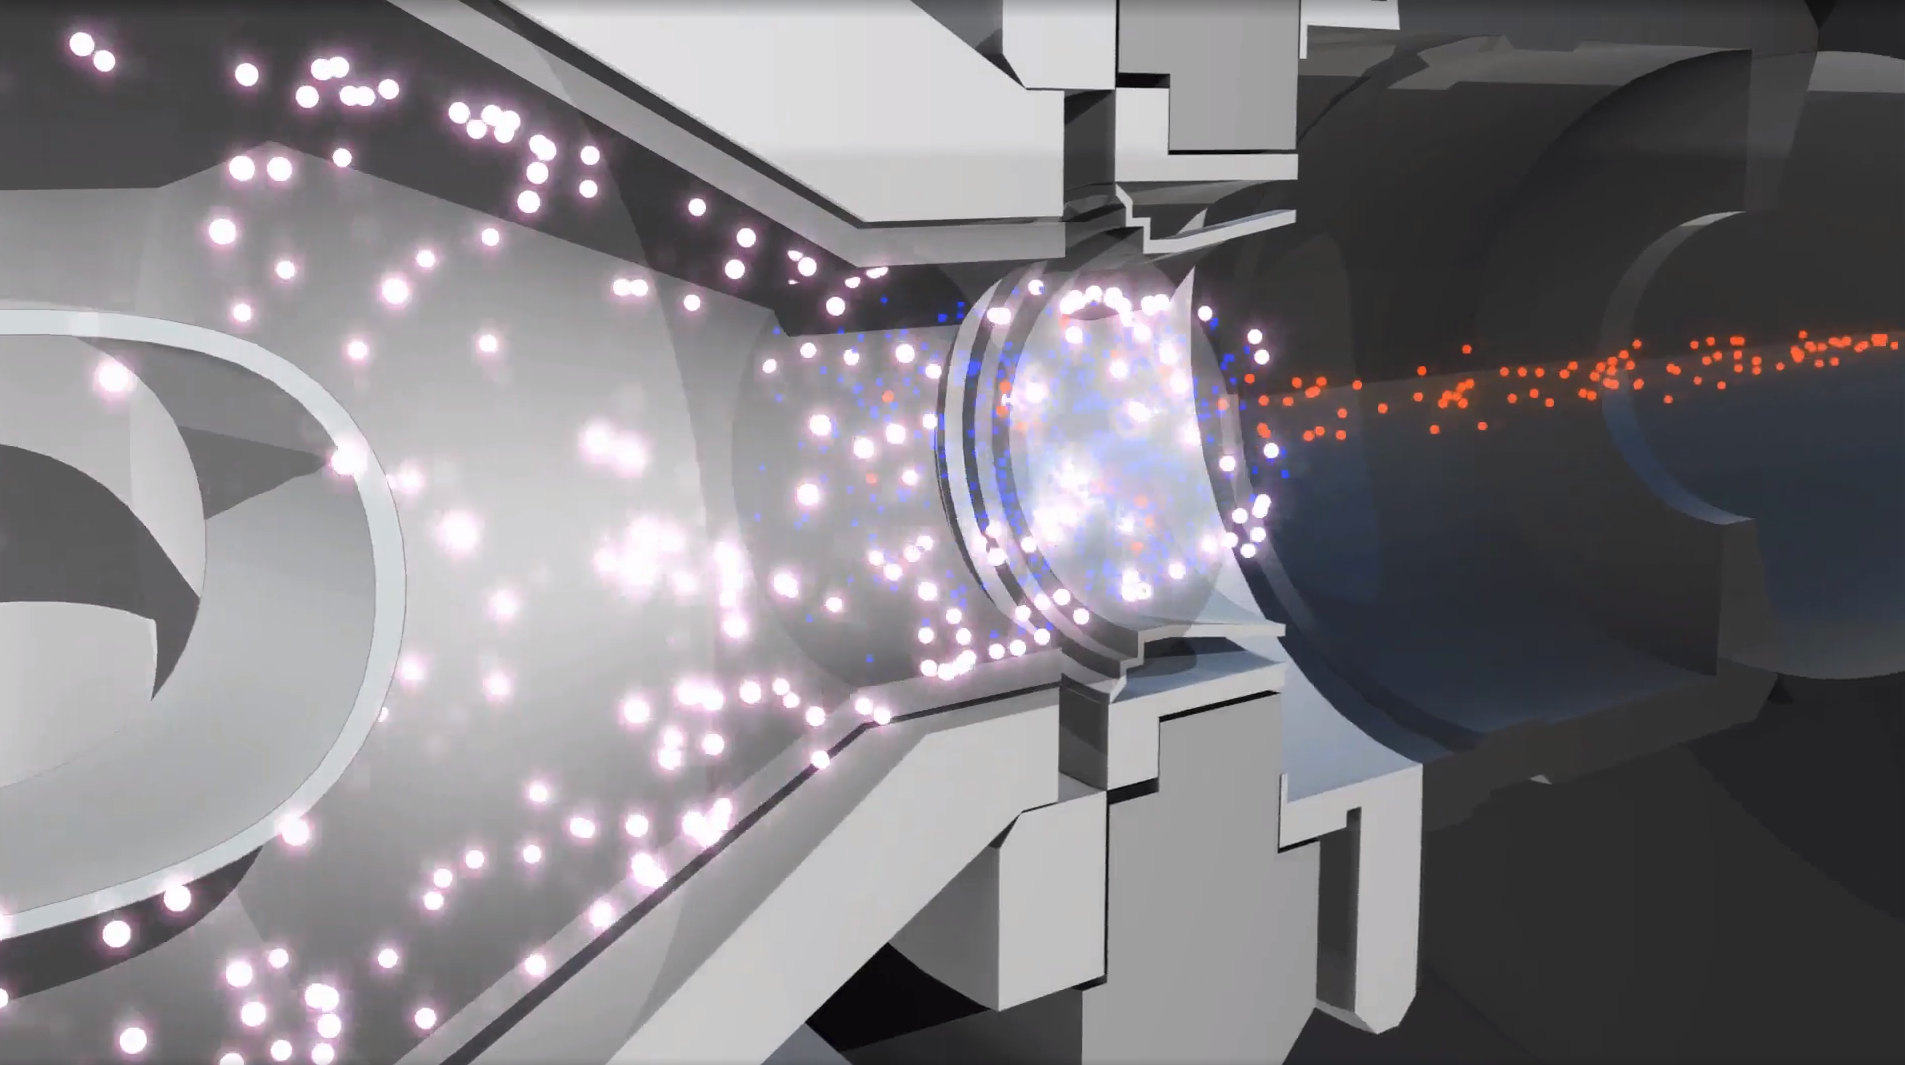
\includegraphics[width=6.0cm,height=3.3cm]{proton_source}\\
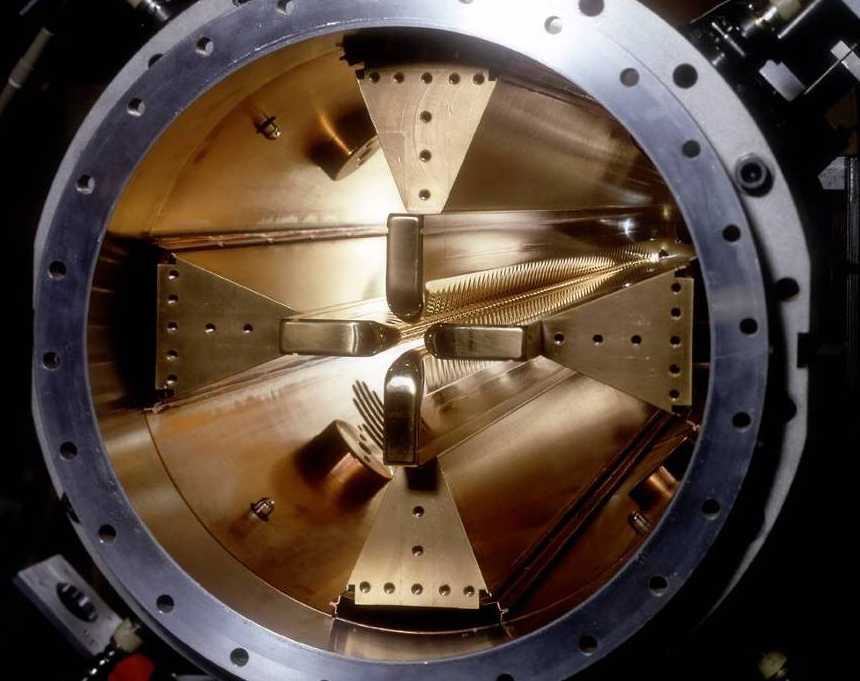
\includegraphics[width=4.5cm,height=3.3cm]{rfq2}
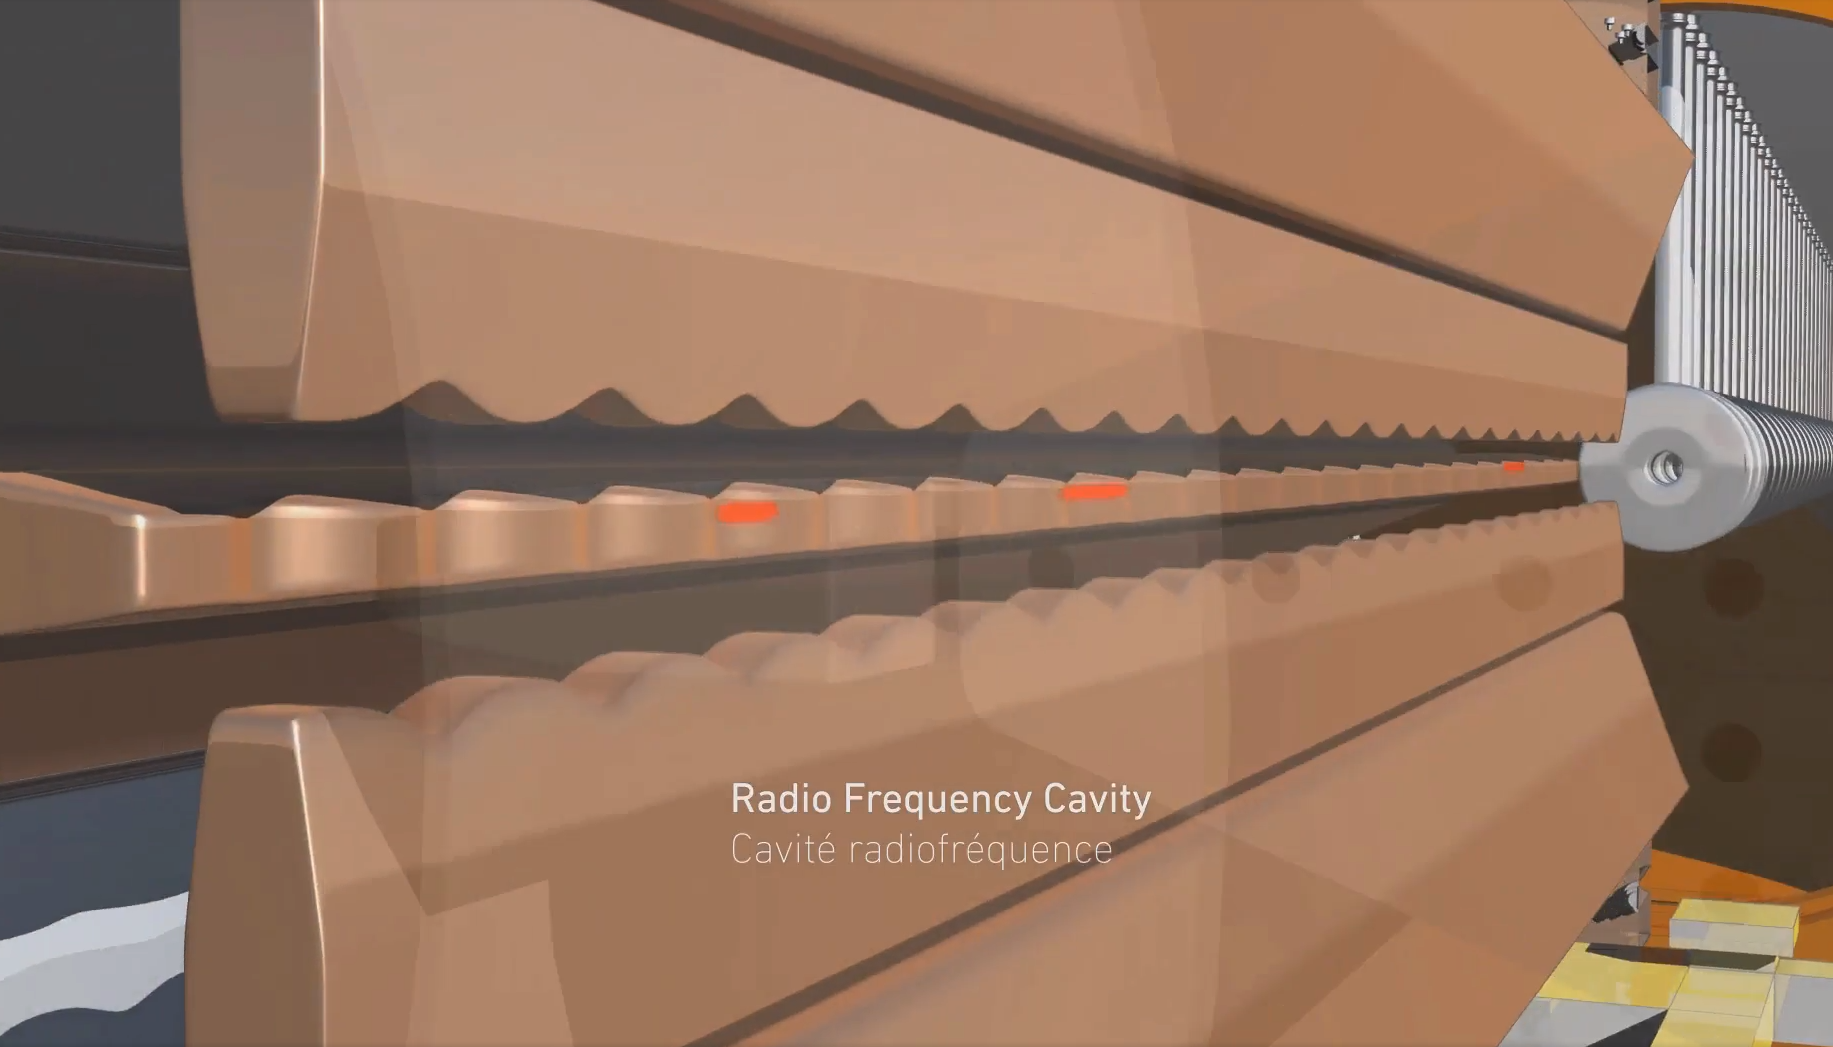
\includegraphics[width=6.0cm,height=3.3cm]{rfq3}
\caption[LHC protons source and first acceleration stage.]{LHC protons source and first acceleration stage. Top: the bottle contains hydrogen gas (white dots) which is injected into the metal cylinder to be broken down into electrons(blue dots) and protons(red dots); Bottom: the obtained protons are directed towards the radio frequency quadrupole which perform the first acceleration, focus the beam and create the bunches of protons.\cite{rfq2,video}}\label{fig:hbottle}
\end{figure}

\noindent In this thesis pp collisions will be considered.\\

\noindent Collection of protons starts with hydrogen atoms taken from a bottle, containing hydrogen gas, and injecting them in a metal cillinder; hydrogen atoms are broken down into electrons and protons by an intense electric field (see figure\ref{fig:hbottle} top). The resulting protons leave the metal cylinder towards a radio frecuency quadrupole (RFQ) that focus the beam, accelerate the protons and create the packets of protons called bunches. In the RFQ, an electric field is generated by a RF wave at a frecuency that matches the resonance frecuency of the cavity where the electrodes are contained. The beam of protons traveling on the RFQ axis experience an alternating electric field gradient that generates the focusing forces.\\

\noindent In order to accelerate the protons, a longitudinal time-variying electric field component is added to the system; it is done by giving the electrodes a sinus-like profile as shown in figure \ref{fig:hbottle} bottom. By matching the speed and phase of the protons with the longitudinal electric field the bunching is performed; protons synchronized with the RFQ (synchronous proton) does not feel an accelerating force, but those protons in the beam that have more (or less) energy than the synchronous proton (asynchronous protons) will feel a decelerating (accelerating) force; therefore, asynchronous protons will oscillate around the synchronous ones forming bunches of protons \cite{rfq}. From the RFQ emerges protons with energy 750 keV in bunches of about $1.15 \times 10^{11}$ protons\cite{lyndon}.        

\begin{figure}[!h]
  \centering
  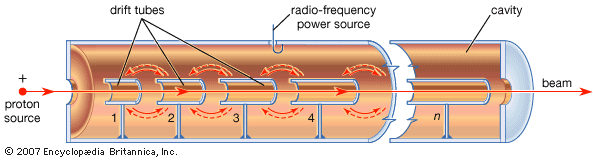
\includegraphics[scale=0.5]{linac}
  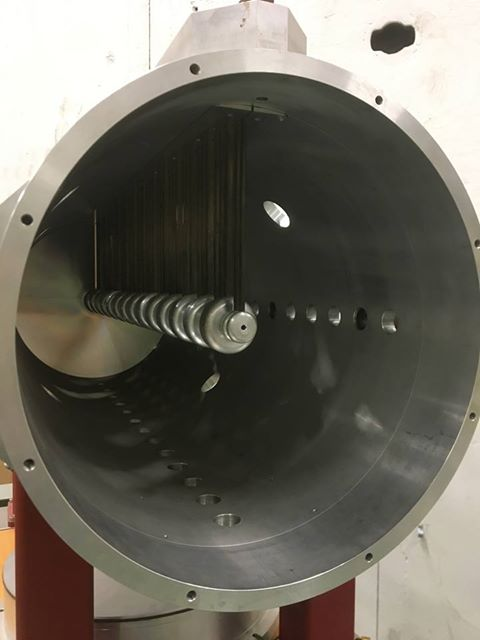
\includegraphics[width=3.0cm,height=3.0cm]{linac2}
  \caption [The LINAC2 accelerating system at CERN.]{The LINAC2 accelerating system at CERN. Radio frecuency (RF) generated electric fields create acceleration and deceleration zones inside the cavity; deceleration zones are blocked by drift tubes where quadrupole magnets focus the proton beam.\cite{linac}}\label{fig:linac}
\end{figure}

\noindent Proton bunches coming from the RFQ goes to the linear accelerator 2 (LINAC2) where they are accelerated to reach 50 MeV energy. In the LINAC2 stage, acceleration is performed using radio frecuency generated electric fields which create zones of acceleration and deceleration as shown in figure \ref{fig:linac}. In the decelerations zones the electric field is blocked using drift tubes where protons are free to drift while quadrupole magnets focus the beam.\\   

\noindent The beam coming from LINAC2 is injected into the proton synchrotron booster (PSB) to reach 1.4 GeV in energy. The next acceleration is provided at the proton synchrotron (PS) up to 26 GeV, followed by the injection into the super proton synchrotron (SPS) where protons are accelerated to 450 GeV. Finally, protons are injected into the LHC where they are accelerated to the target energy of 6.5 TeV.
\noindent PSB, PS, SPS and LHC accelerate protons using the same RF acceleration technic described before. 

\begin{figure}[!h]
\centering
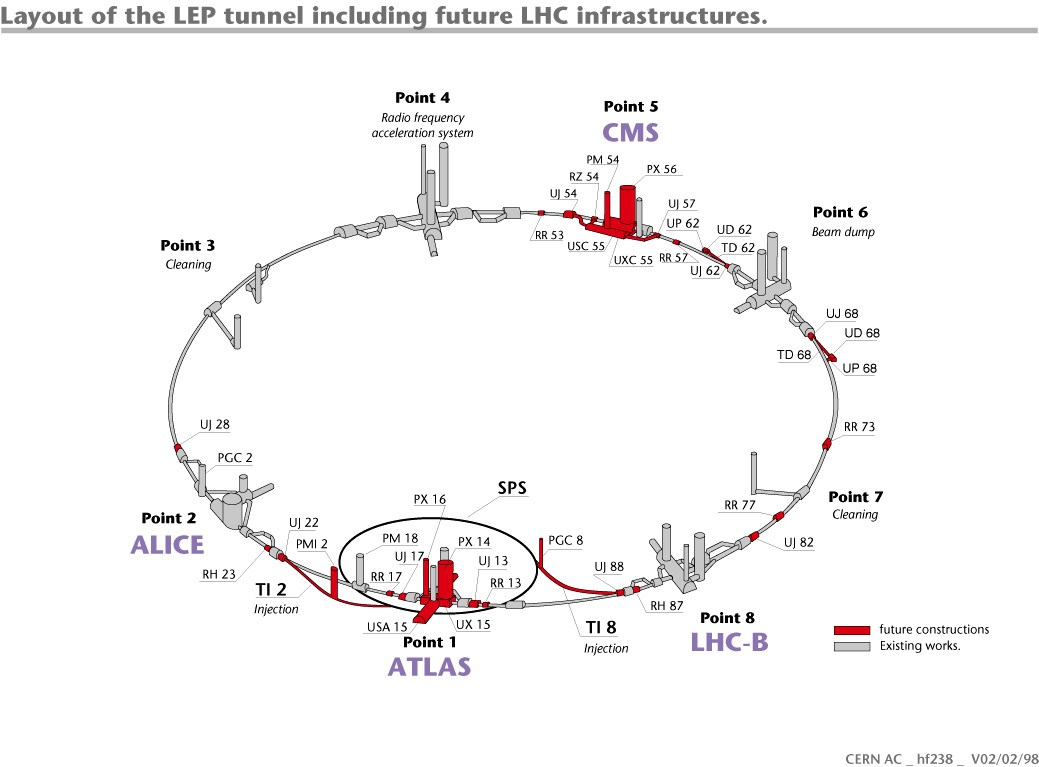
\includegraphics[scale=0.6]{lep}
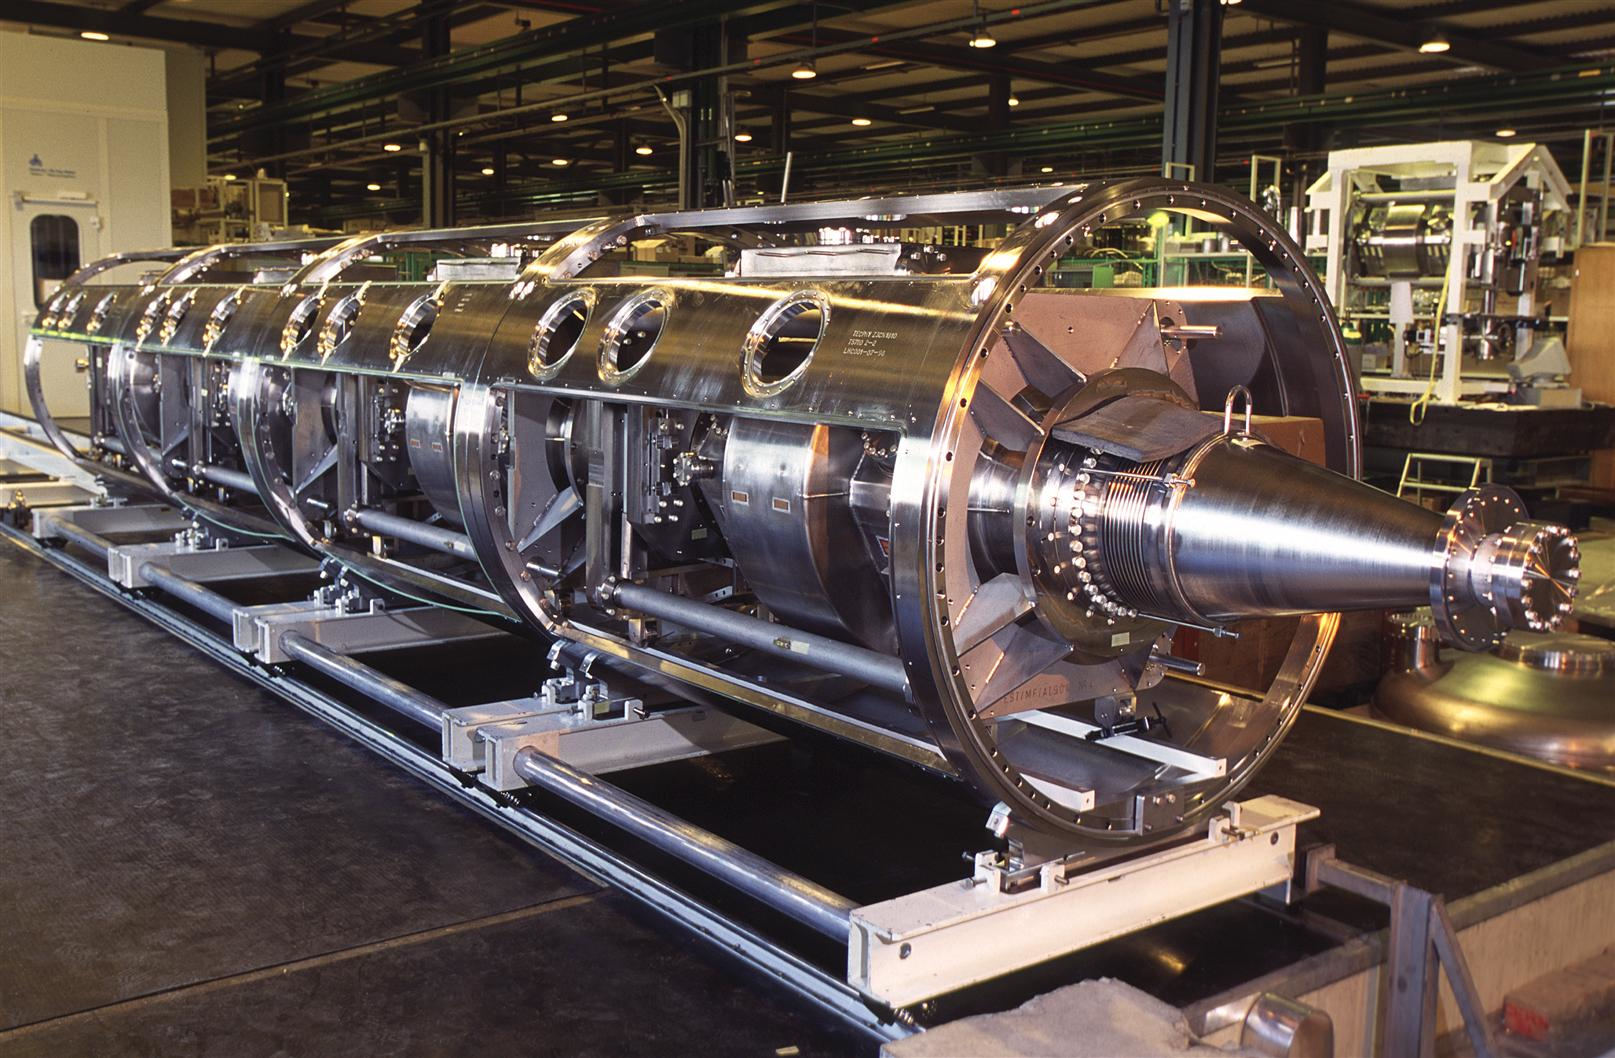
\includegraphics[width=7cm,height=4.2cm]{lhc_rfc}
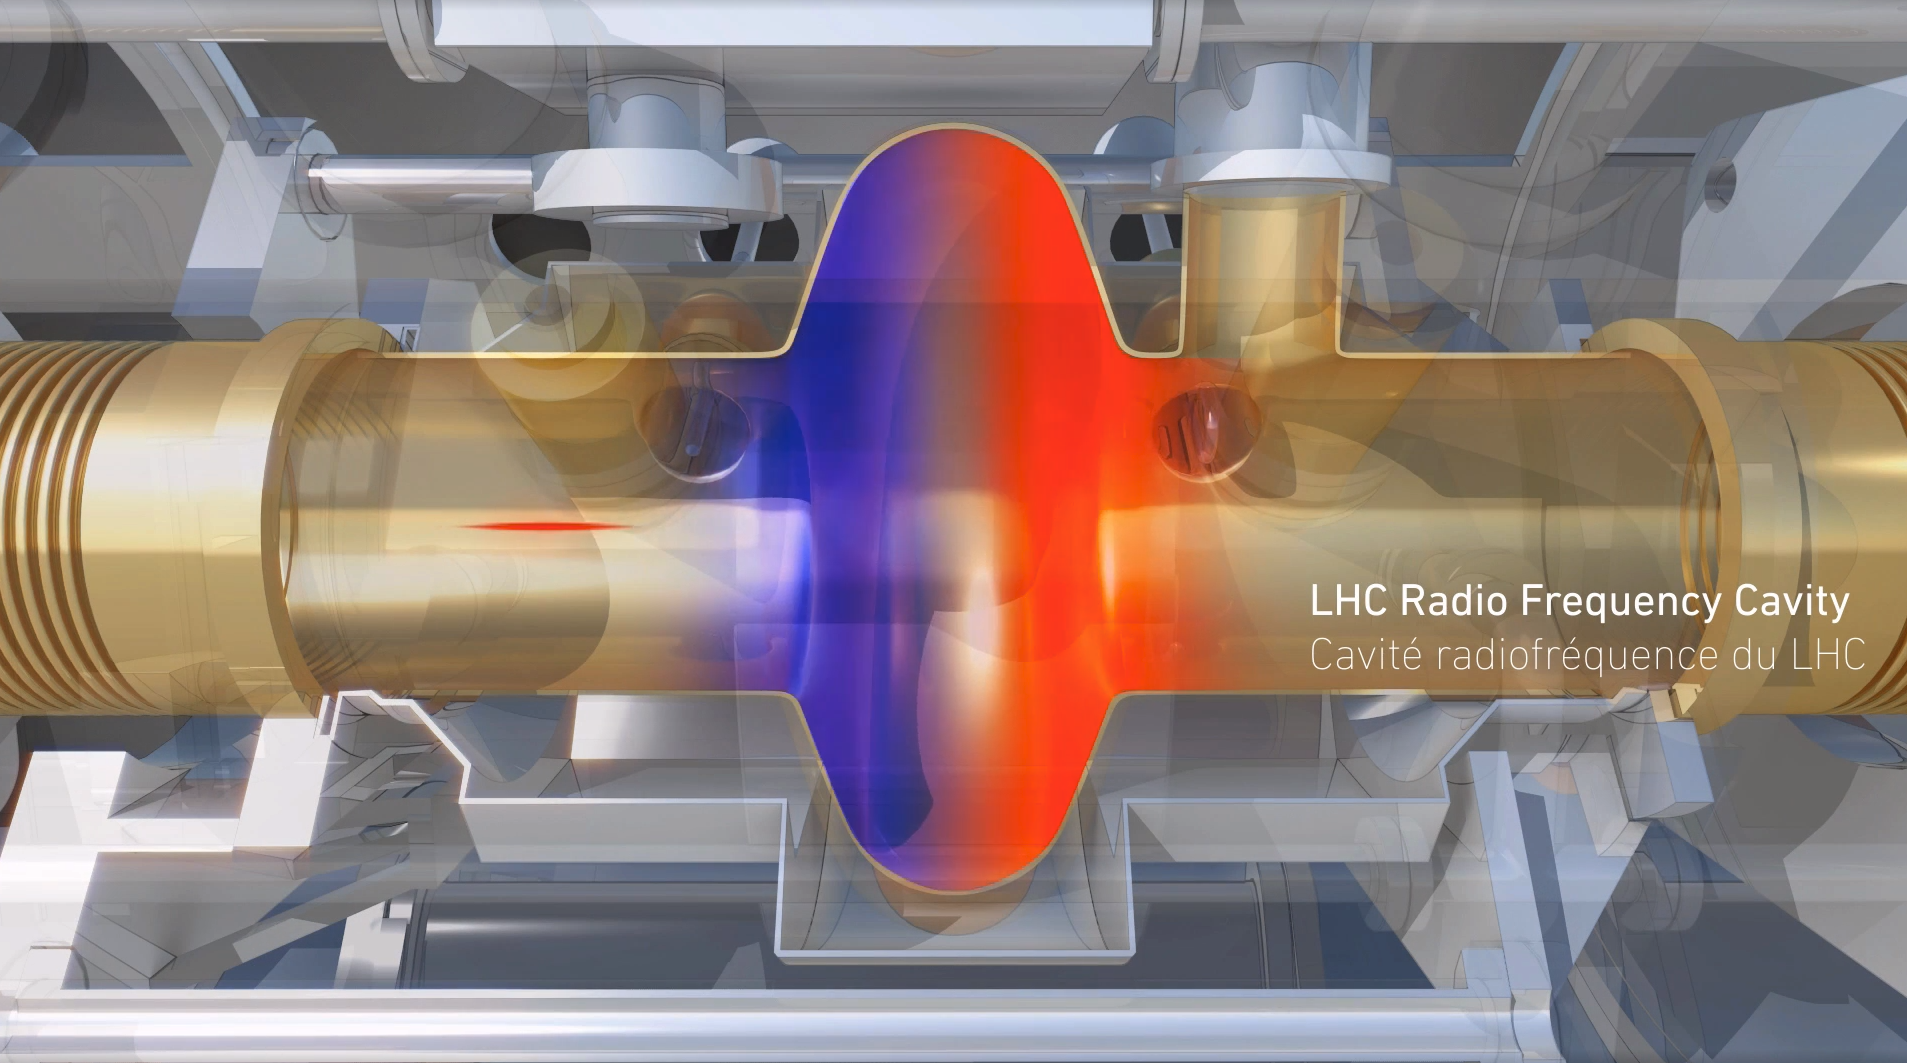
\includegraphics[scale=0.15]{rfc_lhc}
\caption[LHC layout and RF cavities module.]{Top: LHC layout. The red zones indicate the infrastructure additions to the LEP installations, built to accomodate the ATLAS and CMS experiments which exceed the size of the former experiments located there\cite{lep}. Bottom: LHC RF cavities. A module accomodates 4 cavities that accelerate protons and preserve the bunch structure of the beam.\cite{video,lhc_rfc}}\label{fig:lep_rfc}
\end{figure}

\noindent LHC have a system of 16 RF cavities located in the so-called point 4, as shown in figure \ref{fig:lep_rfc} top, tunned at a frecuency of 400 MHz and the protons are carefully timed so additionally to the acceleration effect the bunch structure of the beam is preserved. Bottom side of figure \ref{fig:lep_rfc} shows a picture of a Rf module composed of 4 RF cavities working in a superconducting state at 4.5 K; also is showed a representation of the accelerating electric field that accelerates the protons in the bunch.\\ 

\noindent While protons are accelerated in one section of the LHC ring, where the RF cavities are located, in the rest of their path they have to be kept in the curved trajectory defined by the LHC ring. Technically, LHC is not a perfect circle; RF, injection, beam dumping, beam cleaning and sections before and after the experimental points where protons collide are all straight sections. In total, there are 8 arcs 2.45 Km long each and 8 straight sections 545 m long each. In order to curve the proton's trajectory in the the arc sections, superconducting dipole magnets are used.\\               

\noindent Inside the LHC ring, there are two proton beams traveling in opposite directions in two separated beam pipes; the beam pipes are kept at ultra high vacuum ($\sim 10^{-9}$ Pa) to ensure that there are no particles that interact with the proton beams. The superconducting dipole magnets used in LHC are made of a NbTi alloy, capable of transporting currents of about $12000$ A when cooled at a temperature below 2K using liquid helium (see figure \ref{fig:lhcdipole}).

\begin{figure}[!h]
\centering
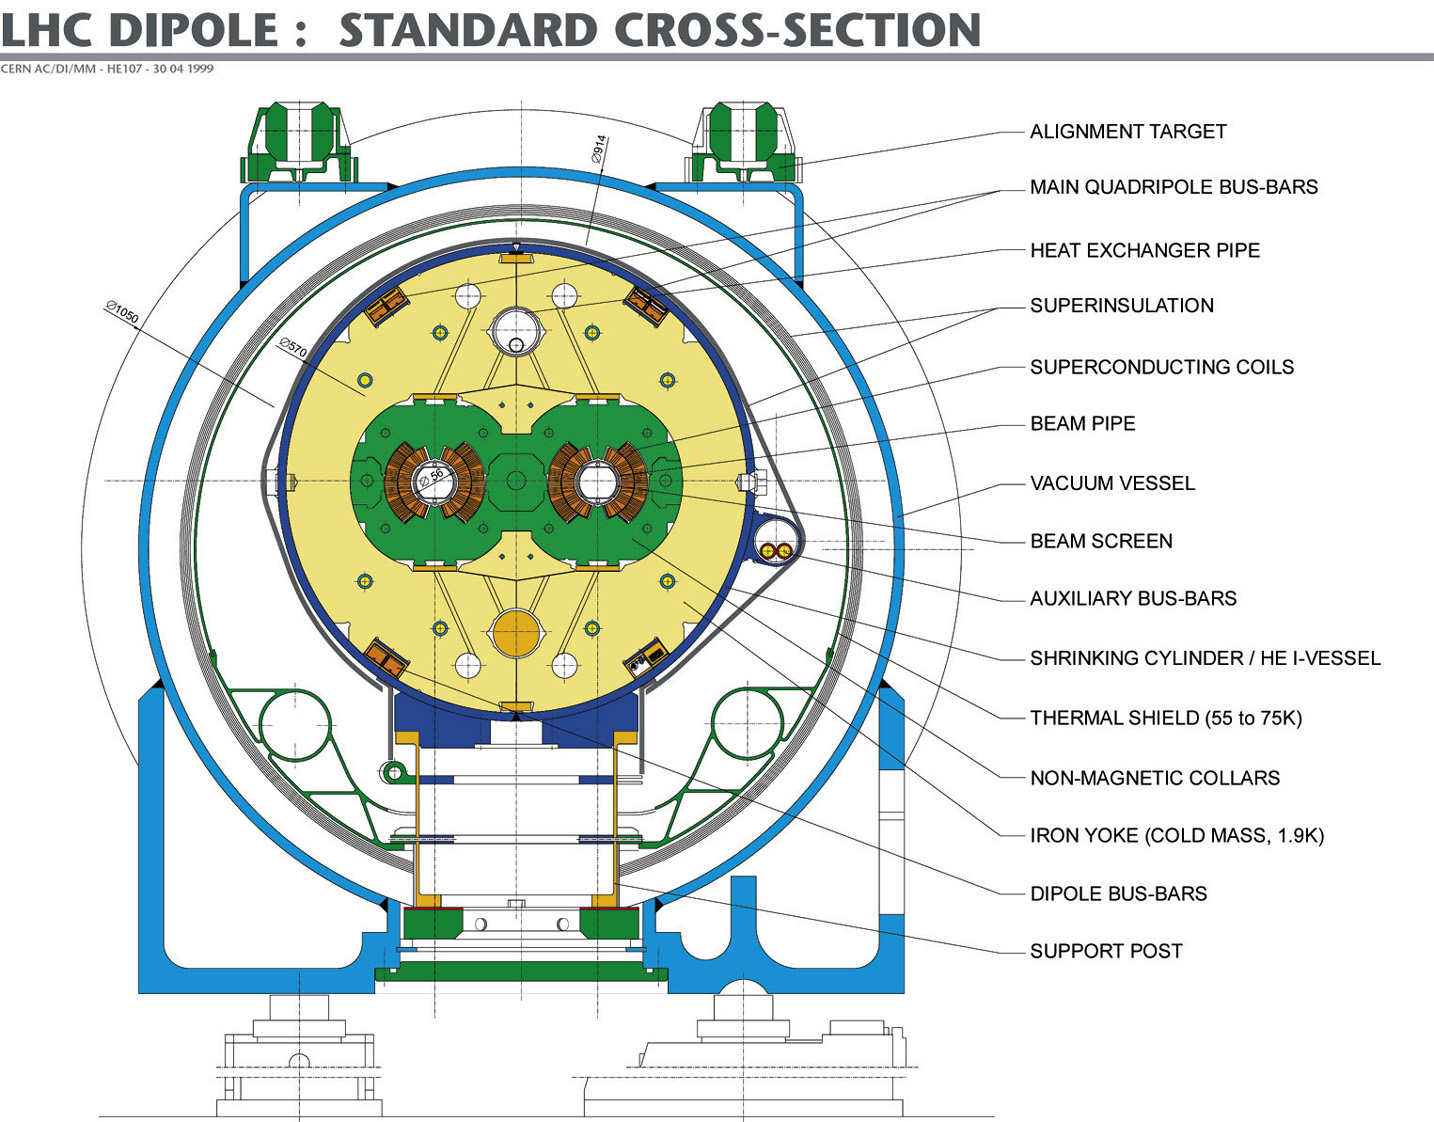
\includegraphics[width=0.7\textwidth]{lhcdipole}
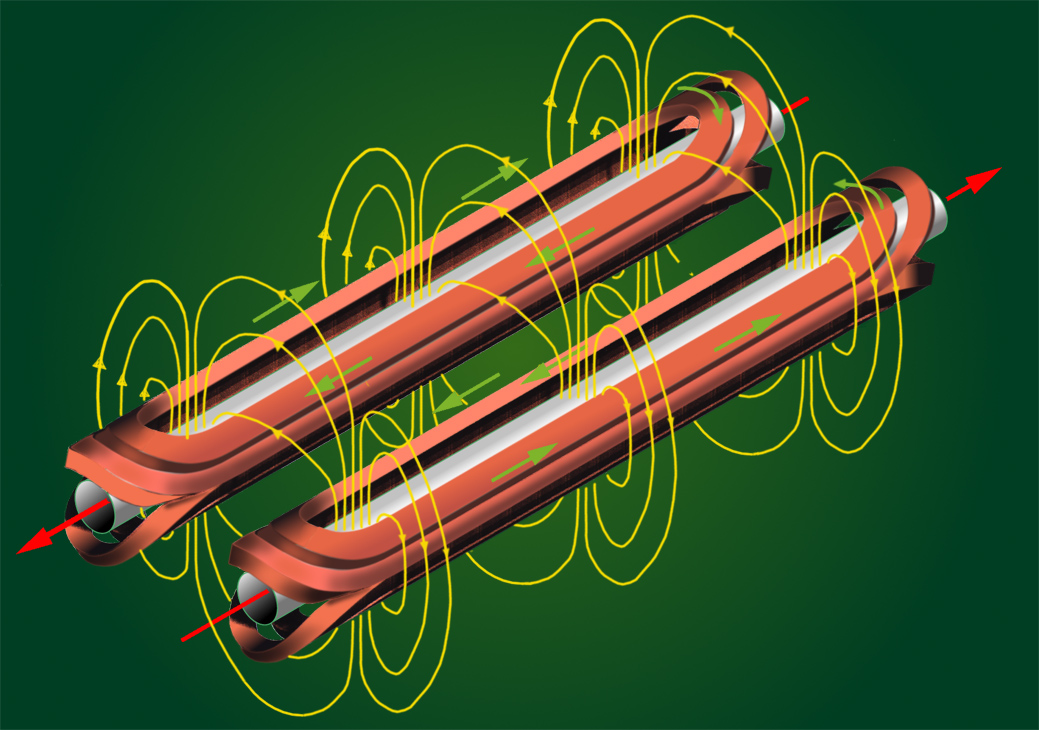
\includegraphics[width=6.0cm,height=4cm]{lhc_dipole2}
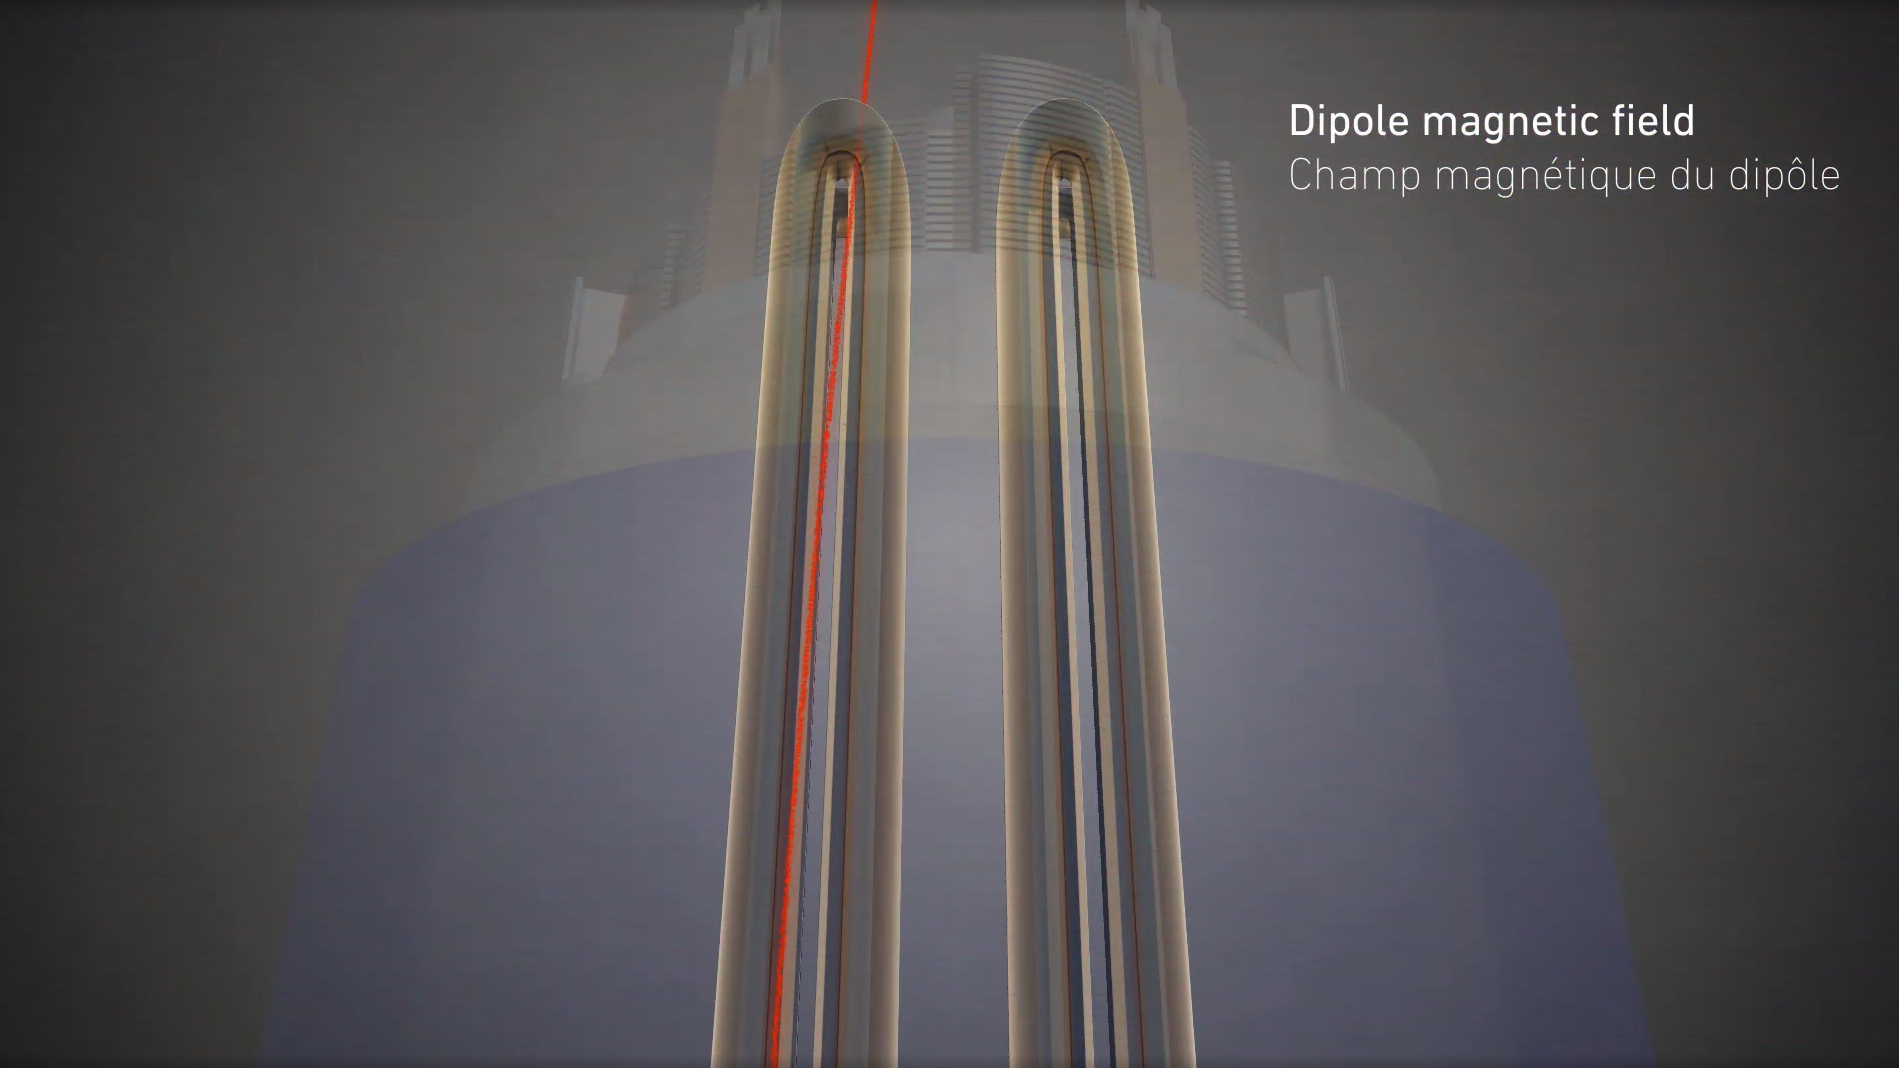
\includegraphics[width=6.0cm,height=4cm]{beam_dev}
\caption [LHC dipole magnet.]{Top: LHC dipole magnet transversal view; cooling, shielding and mechanical support are indicated. Bottom left: Magnetic field generated by the dipole magnets; note that the direction of the field inside one beam pipe is opposite with respect to the other beam pipe which guarantee that both proton beams are curved in the same direction towards the ceneter of the ring. The effect of the dipole magnetic field on the proton beam is represented in the bottom right side \cite{lhc_dipole, dipole_field,video}.}\label{fig:lhcdipole}
\end{figure}

\noindent Protons in the arc sections of LHC feel a centripetal force exerted by the dipole magnets which is perpendicular to the beam trajectory; The magnitude of magnetic field needed can be found assuming that protons travel at $v \approx c$, using the standard values for proton mass and charge and the LHC radius, as
\beqn
F_m=\frac{mv^2}{r}=qBv \quad \to B=8.33 T
\eeqn
\noindent wich is about 100000 times the Earth's magnetic field. A representation of the magnetic field generated by the dipole magnets is shown in the bottom left side of figure \ref{fig:lhcdipole}. The bending effect of the magnetic field on the proton beam is shown in the bottom right side of figure \ref{fig:lhcdipole}. Note that the dipole magnets are not curved; the arc section of the LHC ring is composed of straight dipole magnets of about 15 m. In total there are 1232 dipole magnets along the LHC ring.

\noindent In addition to bending the beam trajectory, the beam has to be focused so it stays in side the beam pipe. The focusing is performed by quadrupole magnets installed in another straight section; in total 858 quadrupole magnets are installed along the LHC ring. Other effects like electromagnetic interaction among bunches, interaction with electron clouds from the beam pipe, gravitational force on the protons, differences in energy among protons in the same bunch, among others, are corrected using sextupole and other magnetic multipoles.     

\noindent The two proton beams inside the LHC ring are made of bunches with a cylindrical shape of about 7.5 cm long and about 1 mm in diameter; when bunches are close to the collision point (CP), the beam is focused up to a diameter of about 16 $\mu$m in order to maximize the luminosity (L) defined as the number of collisions per unit area and per second. Luminosity can be calculated using

\beqn
L=fn\frac{N_1 N_2}{4\pi \sigma_x\sigma_y}
\eeqn

\noindent where f is the revolution frecuency, n is the number of bunches per beam,  $N_1$ and $N_2$ are the number of protons per bunch,  $\sigma_x$ and $\sigma_y$ are the gaussian transverse sizes of the bunches. Using

\begin{align}
  f=&\frac{v}{2\pi r_{LHC}}\approx\frac{3\times10^8m/s}{27km}\approx 11.1 kHz,\nonumber \\
  n=&2808\nonumber \\ 
  N_1=&N_2=1.5\times 10^{11}\nonumber\\
  \sigma_x=&\sigma_y=16\mu m\nonumber
\end{align}
\beqn
L= 1.28\times 10^{34} cm^{-2}s^{-1}
\eeqn

\noindent Luminosity is a fundamental aspect for LHC given that the bigger luminosity, the bigger number of collisions, which means that for processes with a very small cross section the number of expected occurrencies is increased and so the chances of being detected. The integrated luminosty collected by the CMS experiment during 2016 is shown in figure \ref{fig:lumi}; the data analized in this thesis corresponds to an integrated luminosity of 35.9 fb$^{-1}$ at $\sqrt{s}=13$ TeV.

\noindent A way to increase L is increasing the number of bunches in the beam. Currently, the separation between two consecutive bunches in the beam is 7.5 m which corresponds to a time separation of 25 ns. In the full LHC ring the allowed number of bunches is $n=27km/7.5m=3600$; however, there are some gaps in the bunch pattern intended for preparing the dumping and injection of the beam, thus, the proton beams are composed of 2808 bunches. 

\begin{figure}[!h]
\centering
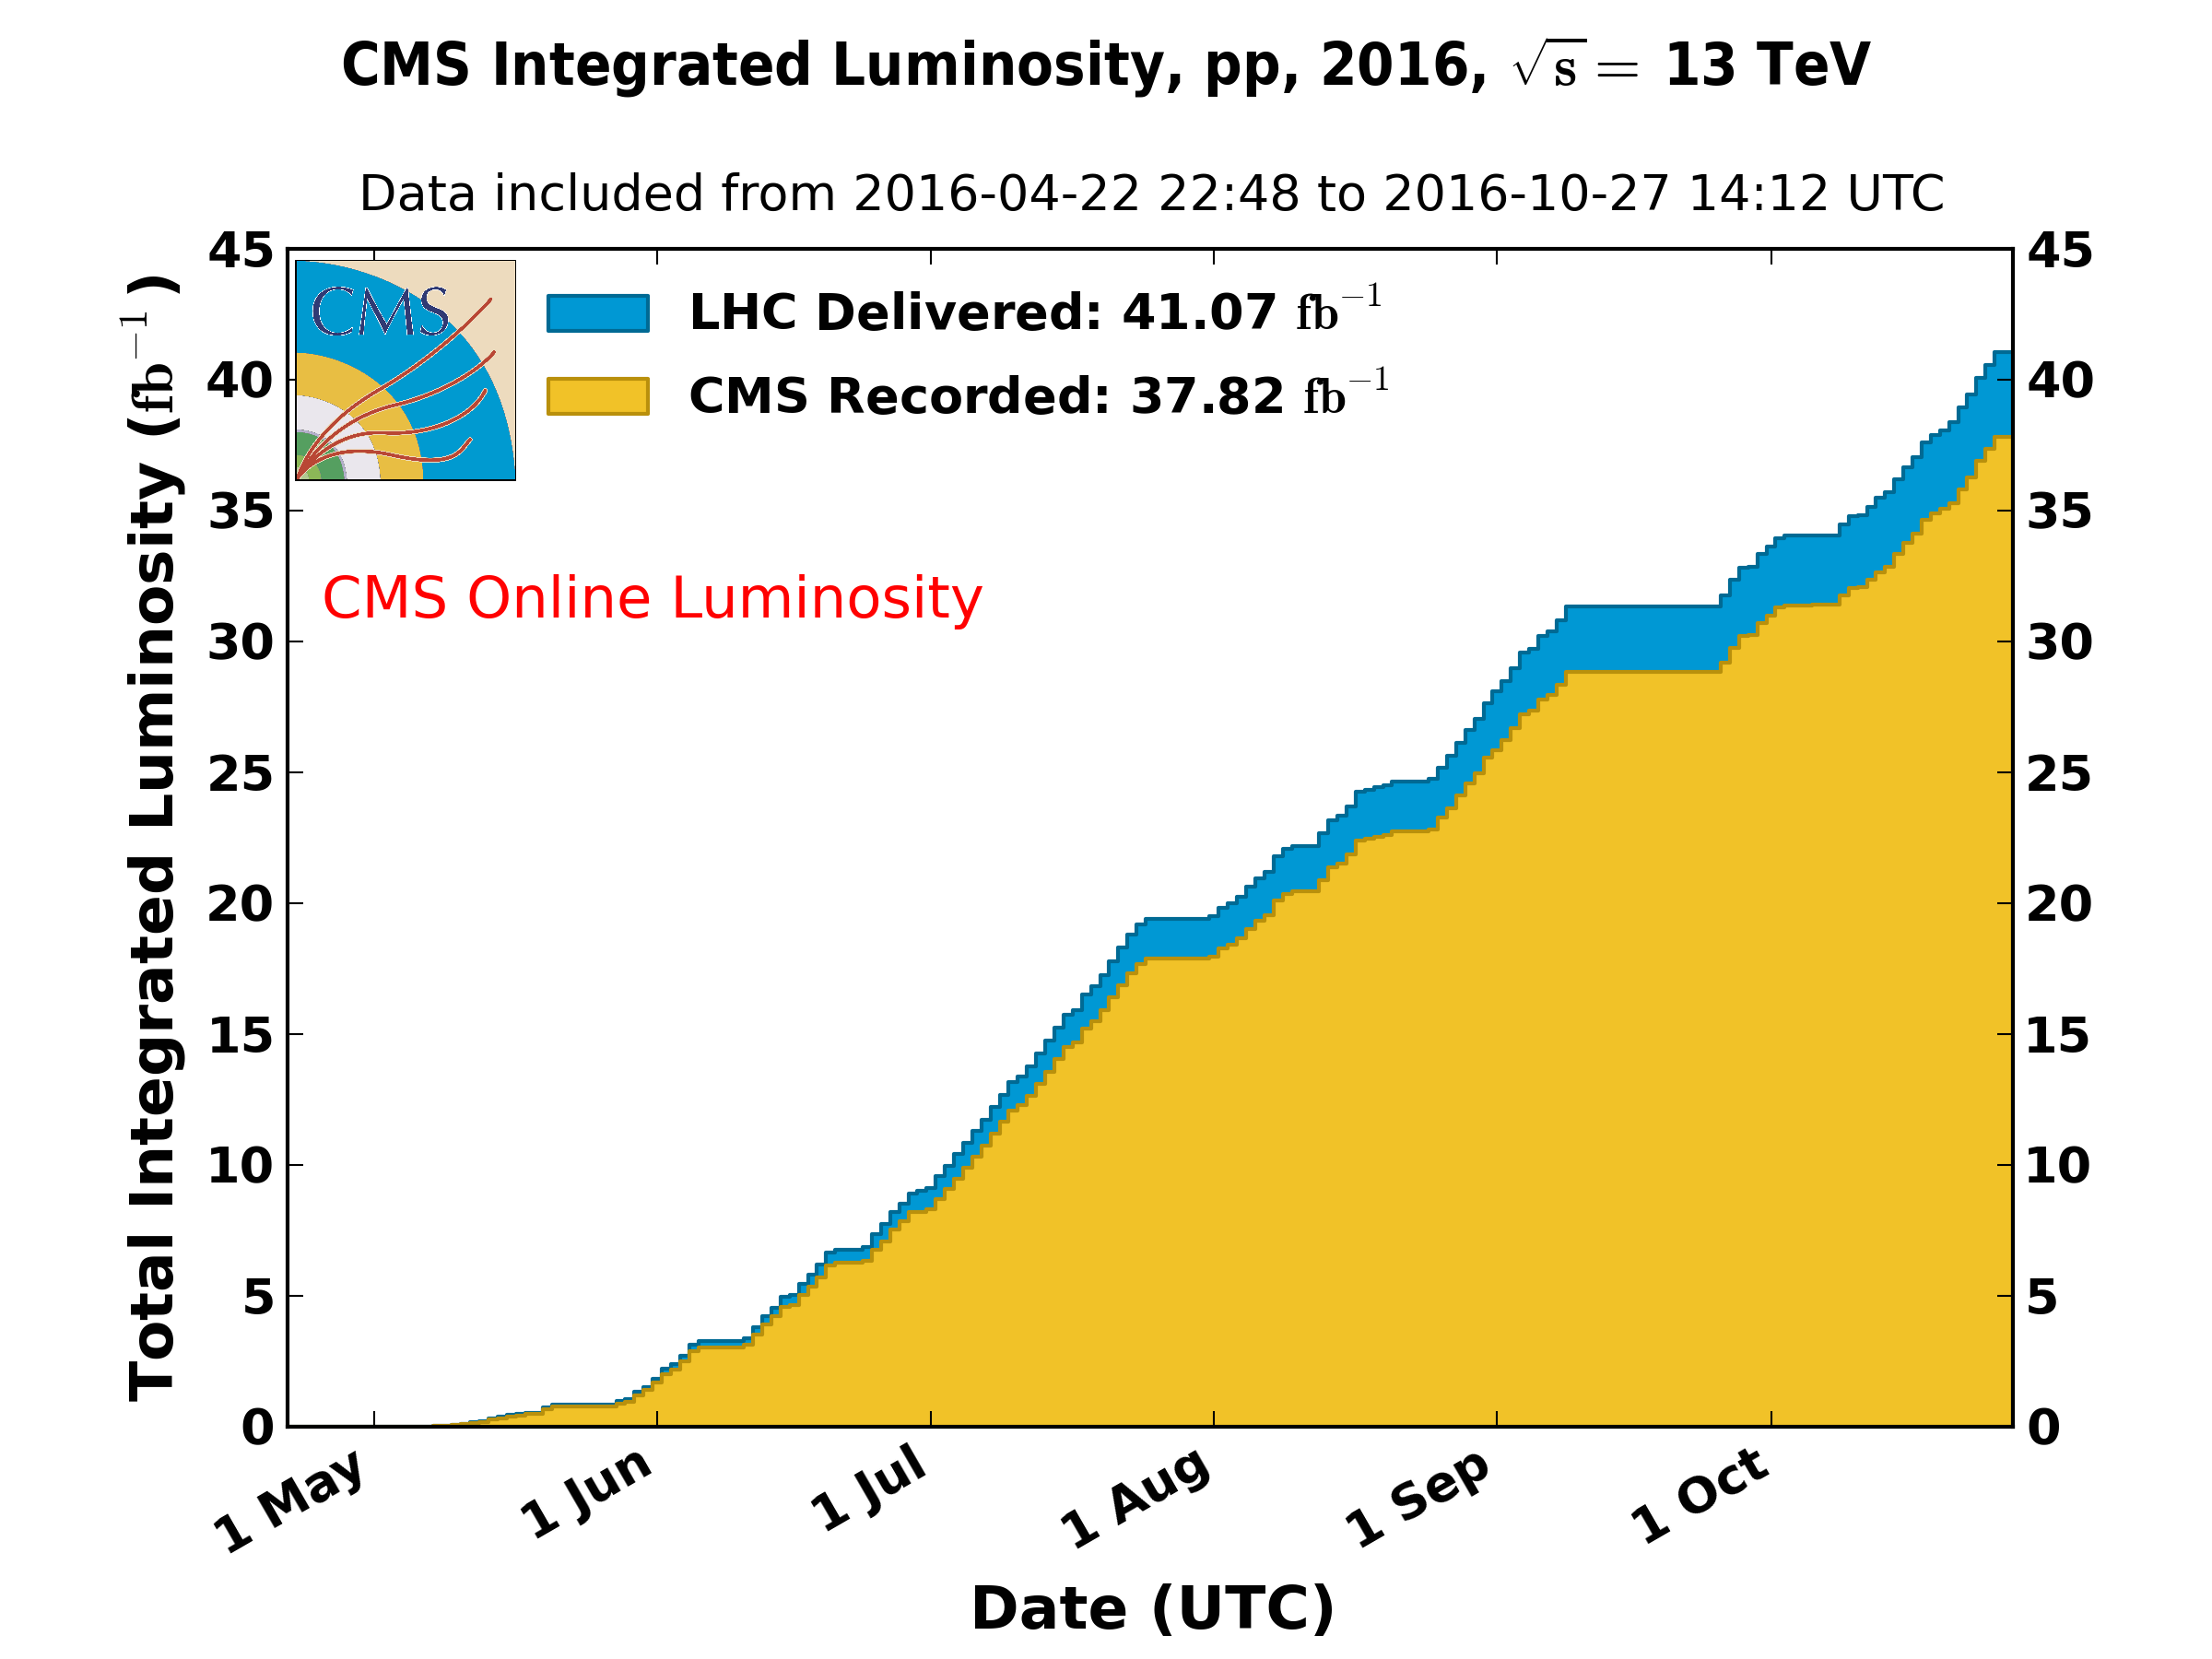
\includegraphics[width=0.7\textwidth]{int_lumi_2016_cms}
\caption [2016 CMS Integrated luminosity]{Integrated luminosity delivered by LHC and recorded by CMS during 2016. The difference between the delivered and the recorded luminosities is due to fails and issues occured during the data taking in the CMS experiment\cite{lumi}.}\label{fig:lumi}
\end{figure}

\noindent Once the proton beams reach the desired energy, they are brought to cross each other producing proton-proton collisions. The bunch crossing happens in precise places where the four LHC experiments are located, as seen in figure \ref{fig:lhc_layout} left. In 2008, the first set of collisions involved protons with $\sqrt{s}=7$ TeV; the energy was increased to 8 TeV in 2012 and to 13 TeV in 2015.

\noindent CMS and ATLAS experiments, which are multi-purpose experiments, are enabled to explore physics in any of the collision modes. LHCb experiment is optimized to explore botom quark physics, while ALICE is optimized for heavy ion collisions searches; TOTEM and LHCf are dedicated to forward physics studies; MoEDAL (not indicated in the figure) is intended for monopoles or massive pseudo stable particles searches.

\begin{figure}[!h]
\centering
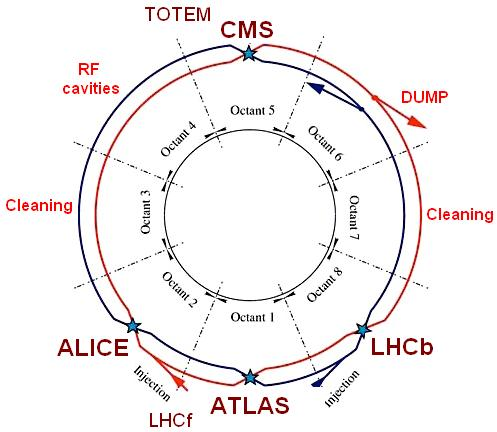
\includegraphics[width=0.55\textwidth]{lhc_layout}
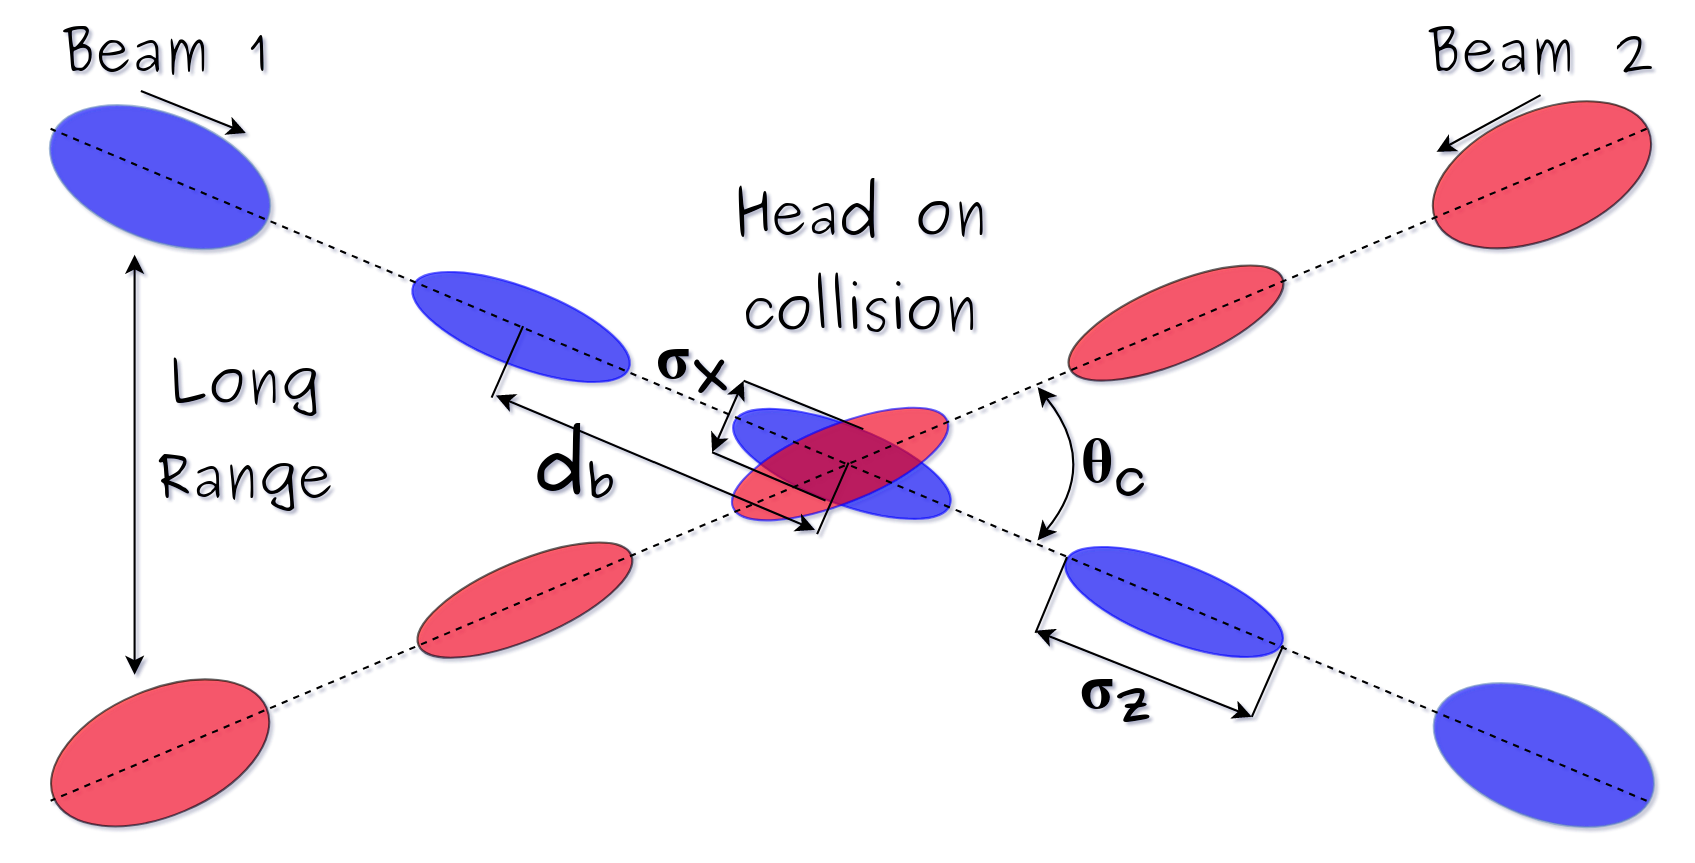
\includegraphics[width=0.4\textwidth]{bcross}
\caption [LHC interaction points]{Left: LHC interaction points. Bunch crossing occurs where the LHC experiments are located \cite{lhc_layout}. Sections indicated as cleaning are dedicated to collimate the beam in order to protect the LHC ring from collisions with protons in very spreaded bunches. Right: bunch crossing scheme. Since the bunch crossing is not perfectly head-on, the luminosity is reduced in a factor of 17\%.}\label{fig:lhc_layout}
\end{figure}

\noindent At the CP there are two interesting details that need to be addressed. The first one is that the bunch crossing does not occur head-on but at a small crossing angle (280 $\mu$rad in CMS and ATLAS) as shown in the right side of figure \ref{fig:lhc_layout}, affecting the overlapping between bunches; the consecuence is a reduction of about 17\% in the luminosity. The second one is occurence of multiple pp collisions in the same bunch crossing; this effect is called pile-up (PU). A fairly simple estimation of the PU follows from estimating the probability of collision between two protons, one from each of the bunches in course of collision; it depends roughly on the ratio of proton size and the cross section of the bunch in the interaction point, \ie,
\beqn
P(pp-collision) \sim \frac{d_{proton}^2}{\sigma_x\sigma_y}=\frac{(1 fm)^2}{(16\mu m)^2} \sim 4\times10^{-21}
\eeqn
\noindent however, there are $N=1.15\times 10^{11}$ protons in a bunch, thus the estimated number of collisions in a bunch crossing is

\beqn
PU= N^2*P(pp-collision)\sim 50  \textrm{  pp-collision per bunch crossing},
\eeqn

\noindent about 20 of those pp collisions are inelastic. Each collision generates a vertex, but only the most energetic is considered as a primary vertex; the rest are considered as PU vertices. A simulation of a multiple pp collision event in a bunch crossing at CMS is showed in figure\ref{fig:pu}. Unstable particles outgoing from the primary vertex will eventually decay; this decay vertex is knon as a secondary vertex.      

\begin{figure}[!h]
\centering
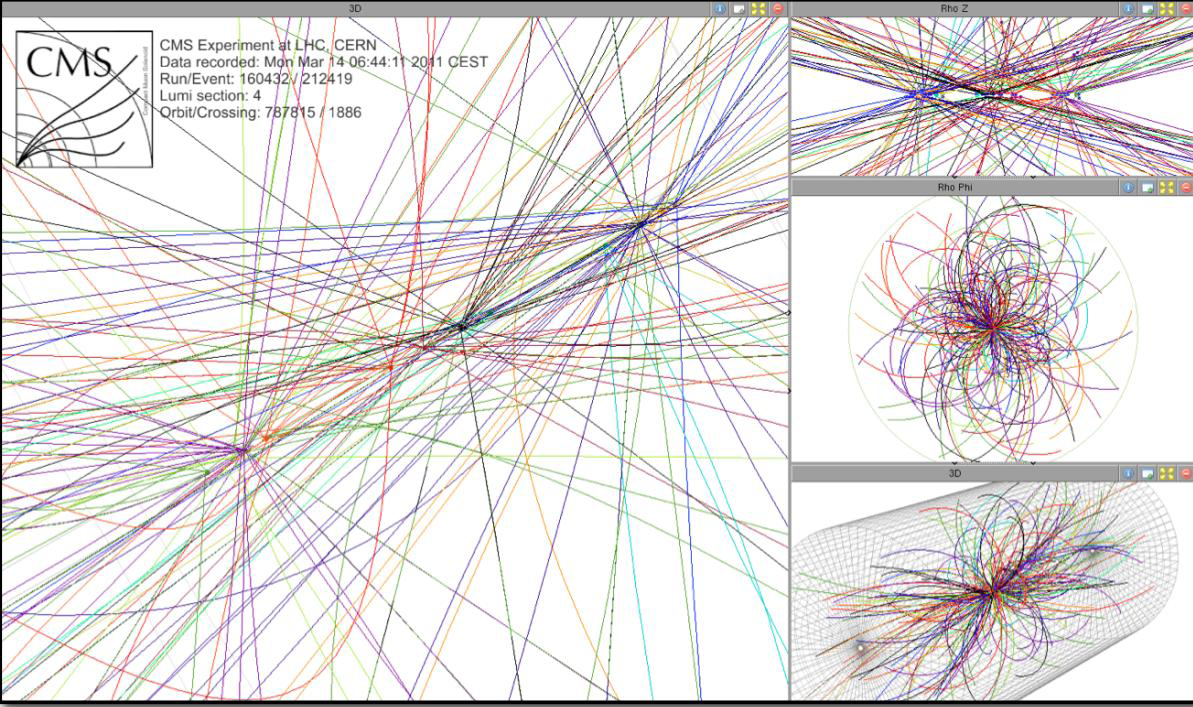
\includegraphics[width=0.65\textwidth]{pu}
\caption [Multiple pp collision bunch crossing at CMS.]{Multiple pp collision bunch crossing at CMS. Only the most energetic vertex is considered and the rets are cataloged as PU vertices \cite{}. }\label{fig:pu}
\end{figure}

\noindent When the beams are exhausted, \ie the number of protons in the bunches is reduced beyond a limit, or in case of emergency, the beams have to be extracted from the beam pipes; the dumping system, in the dump section, perform the extraction safely by directing the beams towards graphite blocks that absorb the beam energy.\\

\noindent Next section present a description of the CMS detector, since it is the detector used to collect the data used in this thesis.


\section{The CMS experiment}

\noindent CMS is a general purpose detector designed to conduct research in a wide range of physics from standard model to new physics like extra dimensions and dark matter. Located at the point 5 in the LHC layout as shown in figure \ref{fig:lep_rfc}, CMS is composed of several detection systems distributed in a cylindrical structure,. In total, CMS weights about 12500 tons in a very compact 21.6 m long and 14.6 m diameter cylinder. It was built in 15 separate sections at the ground level and lowered to the cavern individually to be assembled. A complete and detailed description of the CMS detector and its components is given in reference \cite{cms} on which this section is based in.\\

\noindent Figure \ref{fig:cms} shows the layout of the CMS detector. The design is driven by the requirements on the identification, momentum resolution and unambiguous charge determination of the muons; therefore, a large bending power is provided by the solenoid magnet made of superconducting cable capable to generate a 3.8 T magnetic field. The detection system is composed of (from the innermost to the outermost)

\begin{figure}[!h]
  \centering
  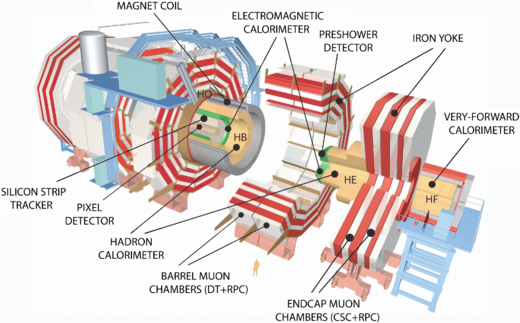
\includegraphics[width=\textwidth]{cms}
  \caption[CMS detector drawing]{CMS detector drawing. The several subdetectors are indicated. The central region of the detector is refferred as the Barrel section while the endcaps are referred as the forward sections. \cite{cms_drawing}.}
  \label{fig:cms}
\end{figure}

\noindent 

\bit
\item Pixel detector.
\item Silicon strip tracker.
\item Preshwoer detector.
\item Electromagnetic calorimeter.
\item Hadronic calorimeter.
\item Muon chambers (Barrel and endcap)
\eit

\noindent The central region of the detector is commonly referred as the barrel section while the endcaps are referred as the forward sections of the detector; thus, each subdetector is composed of a barrel section and a forward section. 


\subsection{Coordinate system}
\noindent The coordinate system used by CMS is centerd in the geometrical center of the detector which is the same as the CP as shown in figure\ref{fig:coord}. The $z$-axis is parallel to the beam direction, while the $Y$-axis pointing vertically upward, and the $X$-axis pointing radially inward toward the center of the LHC.

\begin{figure}[h!]
  \centering
  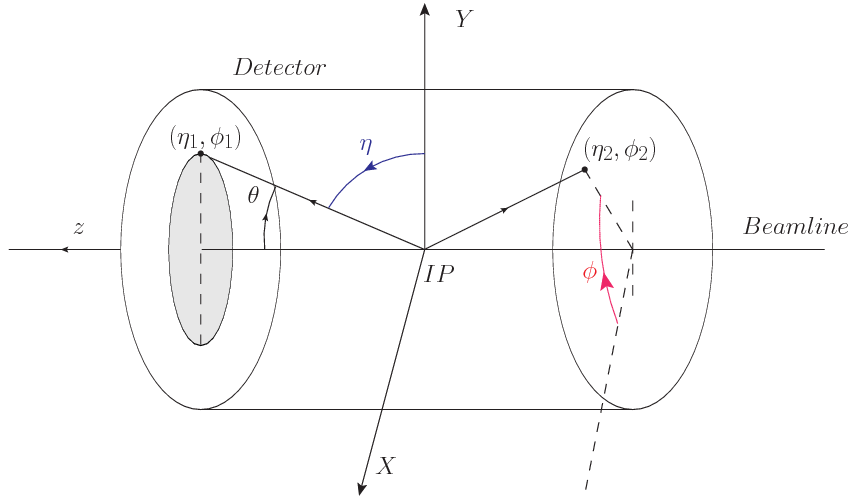
\includegraphics[scale=0.4]{coord}
  \caption[CMS coordinate system]{CMS coordinate system.}
  \label{fig:coord}
\end{figure}

\noindent In addition to the common cartesian and cylindrical coordinate systems, two coordinates are of particular utility in particle physics: rapidity($y$) and pseudorapidity($\eta$), defined in conection to the polar angle $\theta$, energy and longitudinal momentum component (momentum along the $z$-axis) according to

\beqn
y=\frac{1}{2}ln\frac{E+p_z}{E-p_z} \qquad \eta=-ln \left(tan\frac{\theta}{2}\right)
\label{eqn:eta}
\eeqn

\noindent Rapidity is related to the angle between the $XY$-plane and the direction in which the products of a collision are emitted; it has the nice property that the difference between the rapidities of two particles is invariant with respect to Lorents boosts along the $z$-axis. Thus, data analysis becomes more simple when based in rapidity; however, it is not simple to measure the rapidity of higly relativistic particles, as those produced after pp collisions. Under the highly relativistic motion approximation $y$ can be rewritten in terms of the polar angle, arriving to the conclusion that rapidity is approximately equal to the pseudorapidity defined above, \ie $y\approx\eta$. Note that $\eta$ is easier to measure that $y$ given the direct relationship between the former and the polar angle. Angular distance between two objects in the detector ($\Delta R$) is defined in terms of their coordinates $(\eta_1,\phi_1)$, $(\eta_2,\phi_2)$ as
\beqn
\Delta R = \sqrt{(\Delta\eta)^2 - (\Delta\phi)^2 }
\eeqn

\subsection{Pixels detector}

\noindent  The CMS tracking system is designed to provide a precise measurement of the trajectory followed by the charged particles created after the pp collisions as; also, the precise reconstruction of the primary and secondary vertices is expected in an environment where, each 25 ns, the bunch crossing produce about 20 inelastic collisions and about 1000 particles. An increment in the luminosity is ongoing which implies that the PU will increase accordingly. \\

\noindent The pixel detector was replaced during the 2016-2017 year end shut down, due to the increasingly challenging operation conditions like the higher particle flow and more radiation harsh environment among others. The new one is responding as expected, reinforcing its crucial role in the successful way to fullfil the new LHC physics objetives after the discovery of the Higgs boson. The last chapter of this thesis is dedicated to describe my contribution to the `` Forward Pixel Phase 1 upgrade''.\\

\noindent  The current pixel detector is composed of 1856 silicon pixel detector modules organized in four barrel layers in the central region and three disks in the forward region; it is designed to record efficiently and with high precision, up to 10$\mu$m in the $XY$-plane and 20$\mu$m in the $z$-direction, the first four space-points near to the CP region (see figure \ref{fig:pixel_tracker} left side) in the range $|\eta|\leq 2.5$. The first barrel layer is located at a radius of 30 mm from the beamline, while the fourth layer is located at a radius of 160 mm closer to the strip tracker innner barrel layer (see section \ref{sst}) in order to reduce the rate of fake tracks. The high granularity of the detector is represented in its about 123 Mpixels, each of size $100\times150\mu$m$^2$, which is almost twice the channels of the old detector. The transverse momentum resolution of tracks can be measured with a resolution of 1-2\% for muons of $p_T=100$ GeV. \\

\begin{figure}[h!]
  \centering
  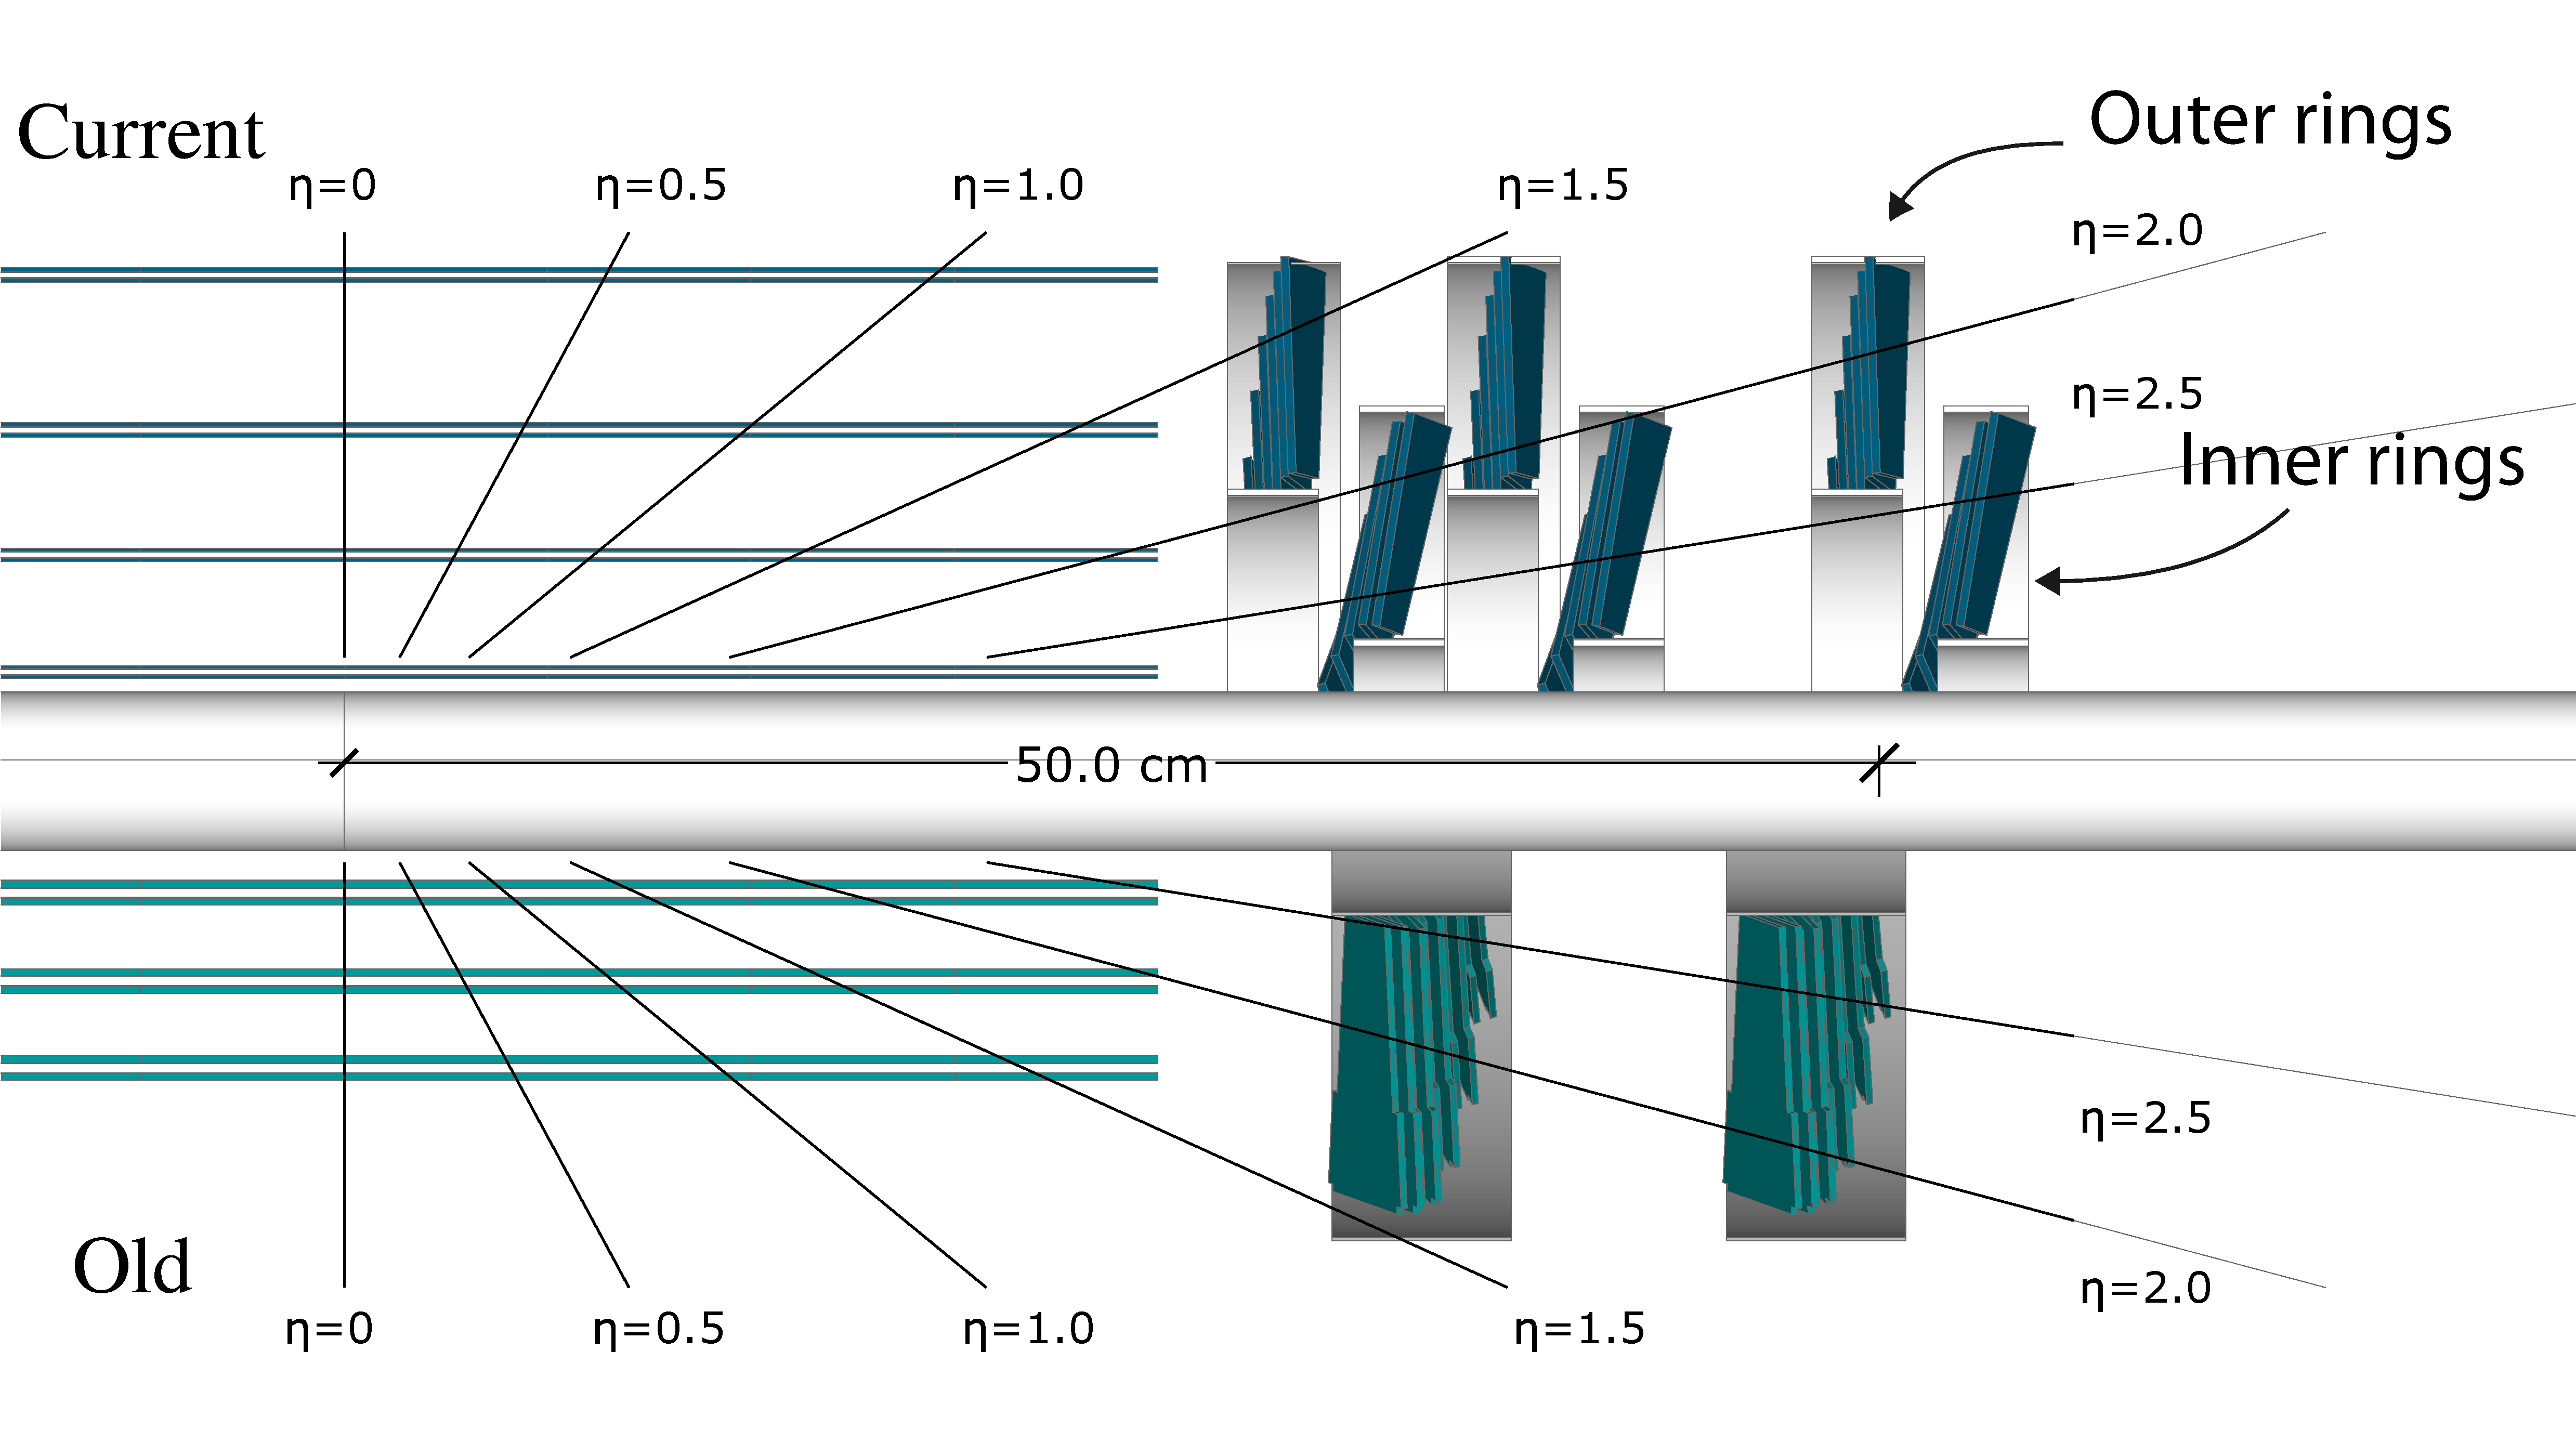
\includegraphics[width=9.5cm]{fpix1}
  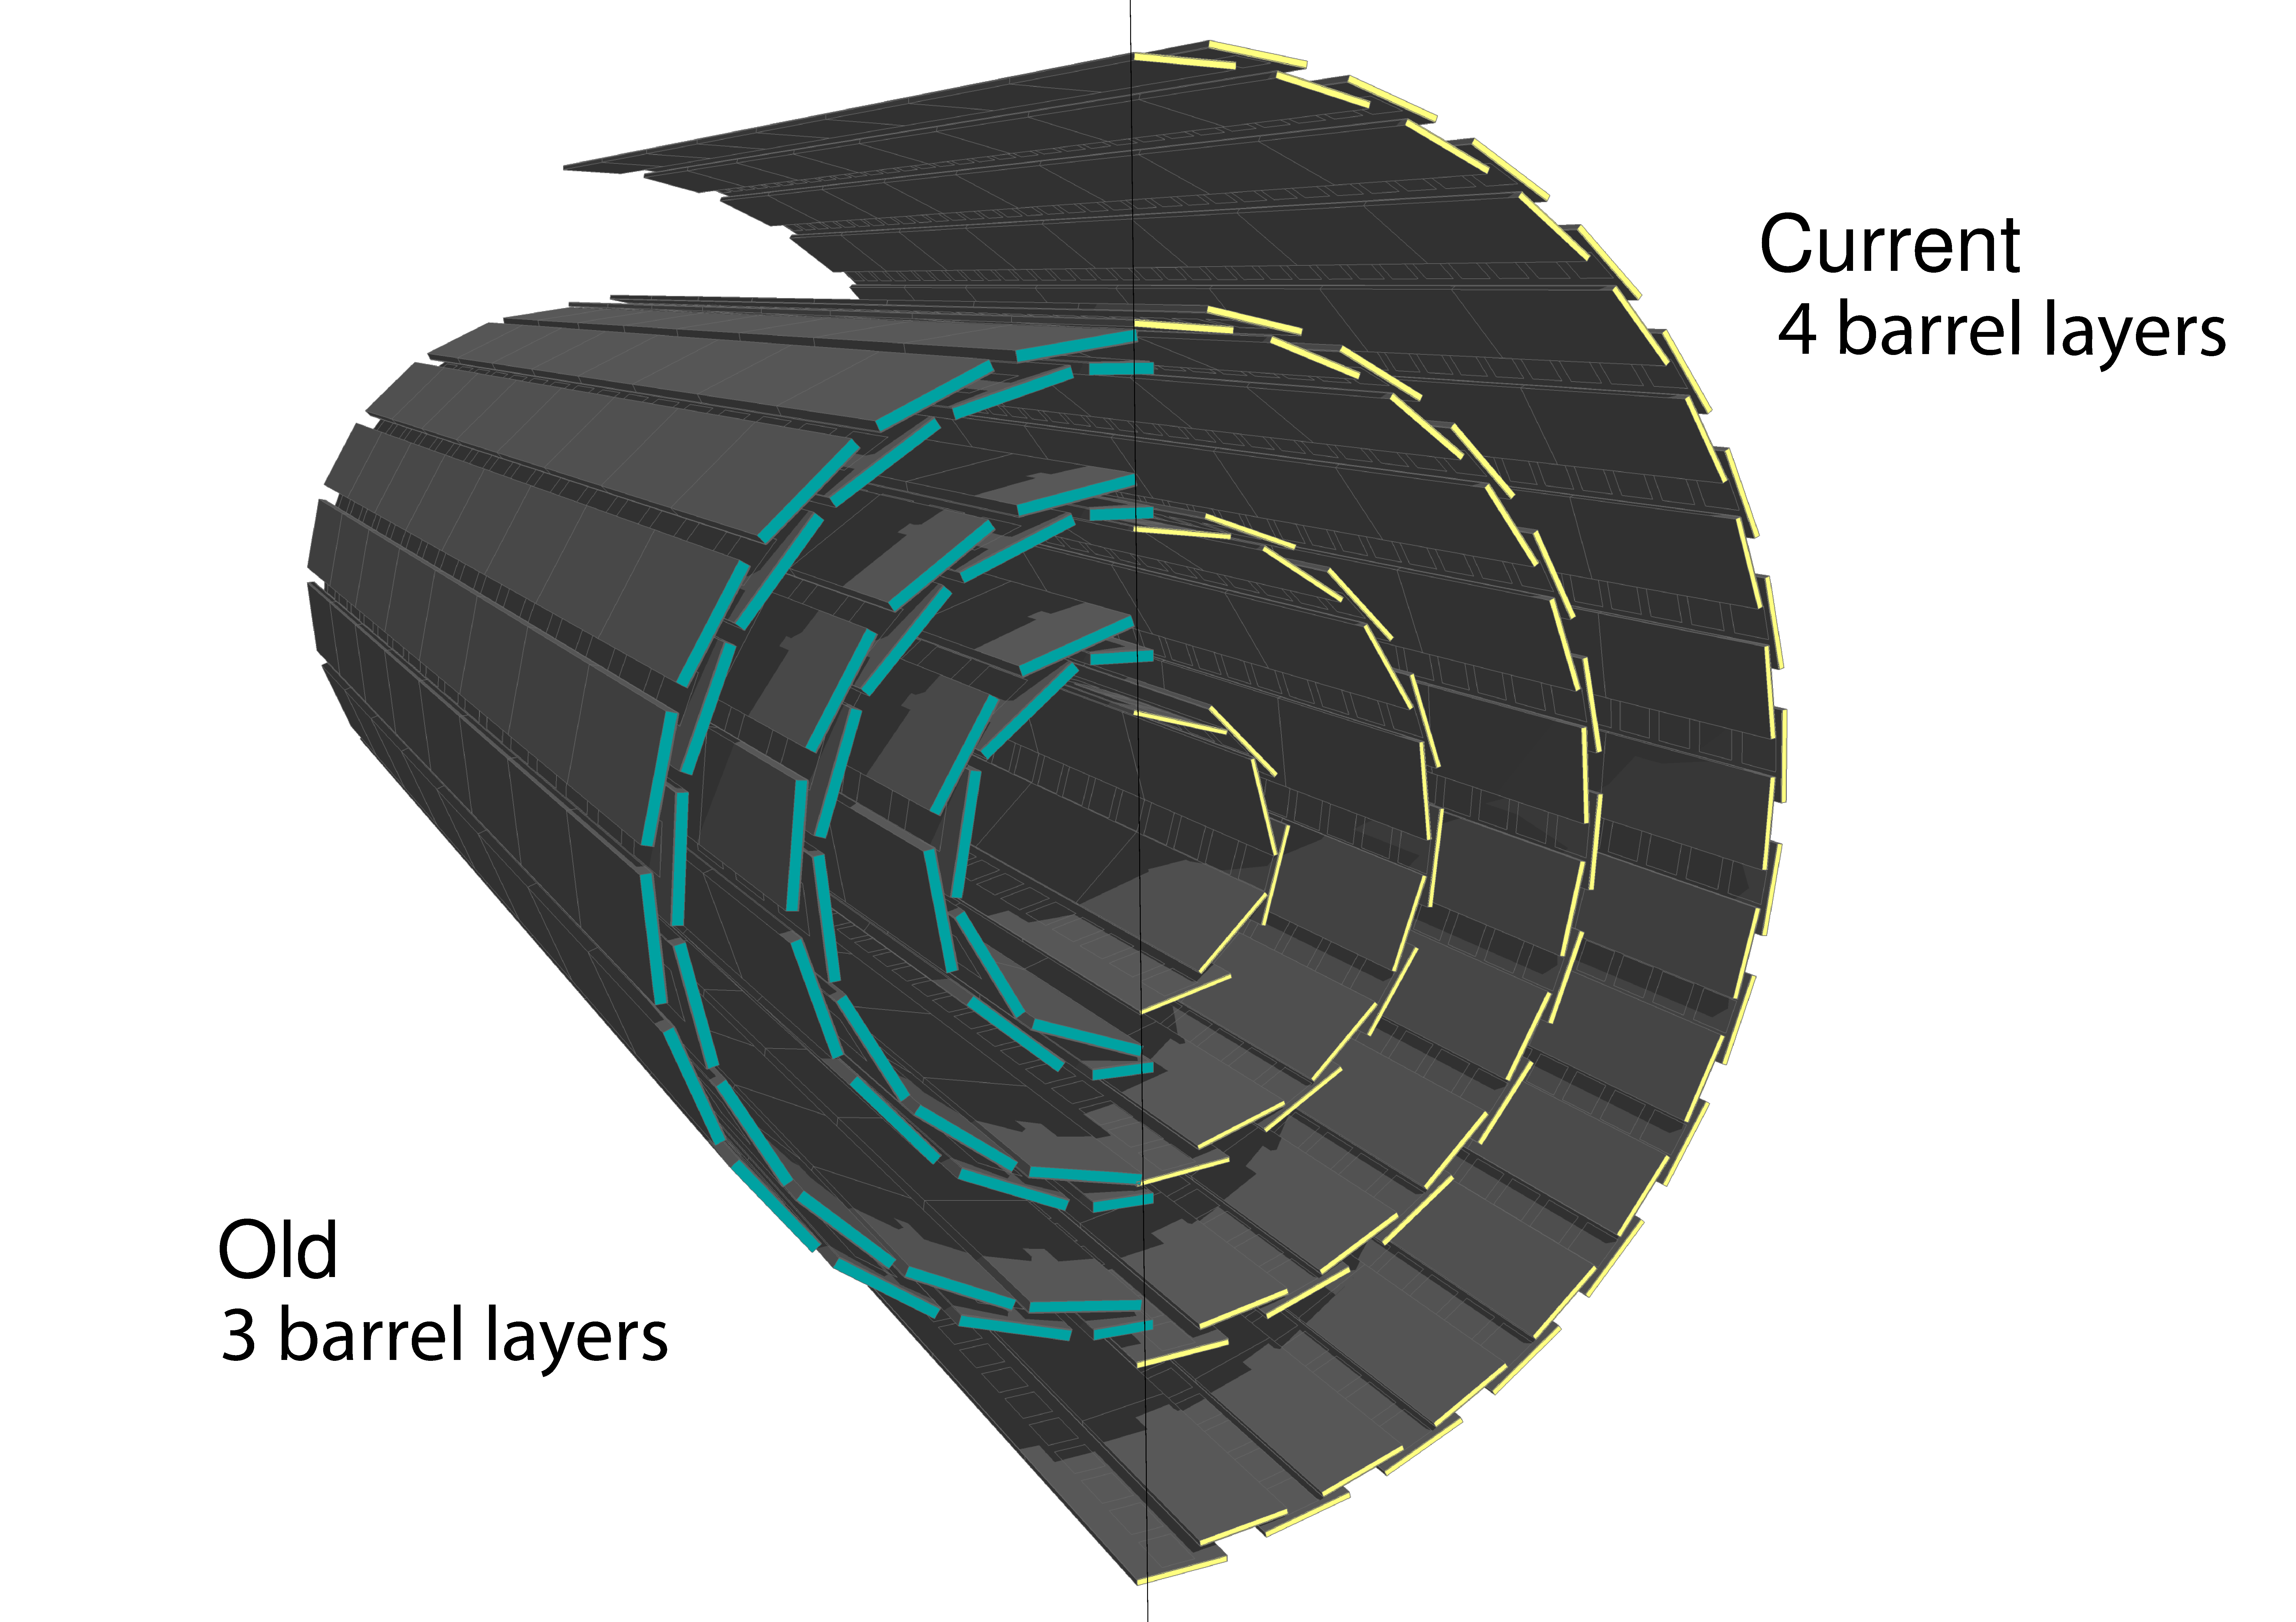
\includegraphics[width=5.5cm]{bpix1}
  \caption[CMS pixel detector schematic view.]{CMS pixel detector schematic view. Left: layout comparing the layers and disks in the old and current pixel detectors. Right: Transverse-oblique view comparing the pixel barrel layers in the two \cite{pix_tdr}.}
  \label{fig:pixel_tracker}
\end{figure}

\noindent Some of the improvements with respect to the previous pixel detector include a higher average tracking efficiency and lower average fake rate as well as higher track impact parameter resolution which is fundamental in order to increase the efficiency in the identification of jets originating from b quarks (b-tagging). A significant source of improvement comes from the overall reduction in the material budget of the detector which results in less photon conversions and less multiple scattering from charged particles.    

\subsection{Silicon strip tracker}\label{sst}
\begin{figure}[h!]
  \centering
  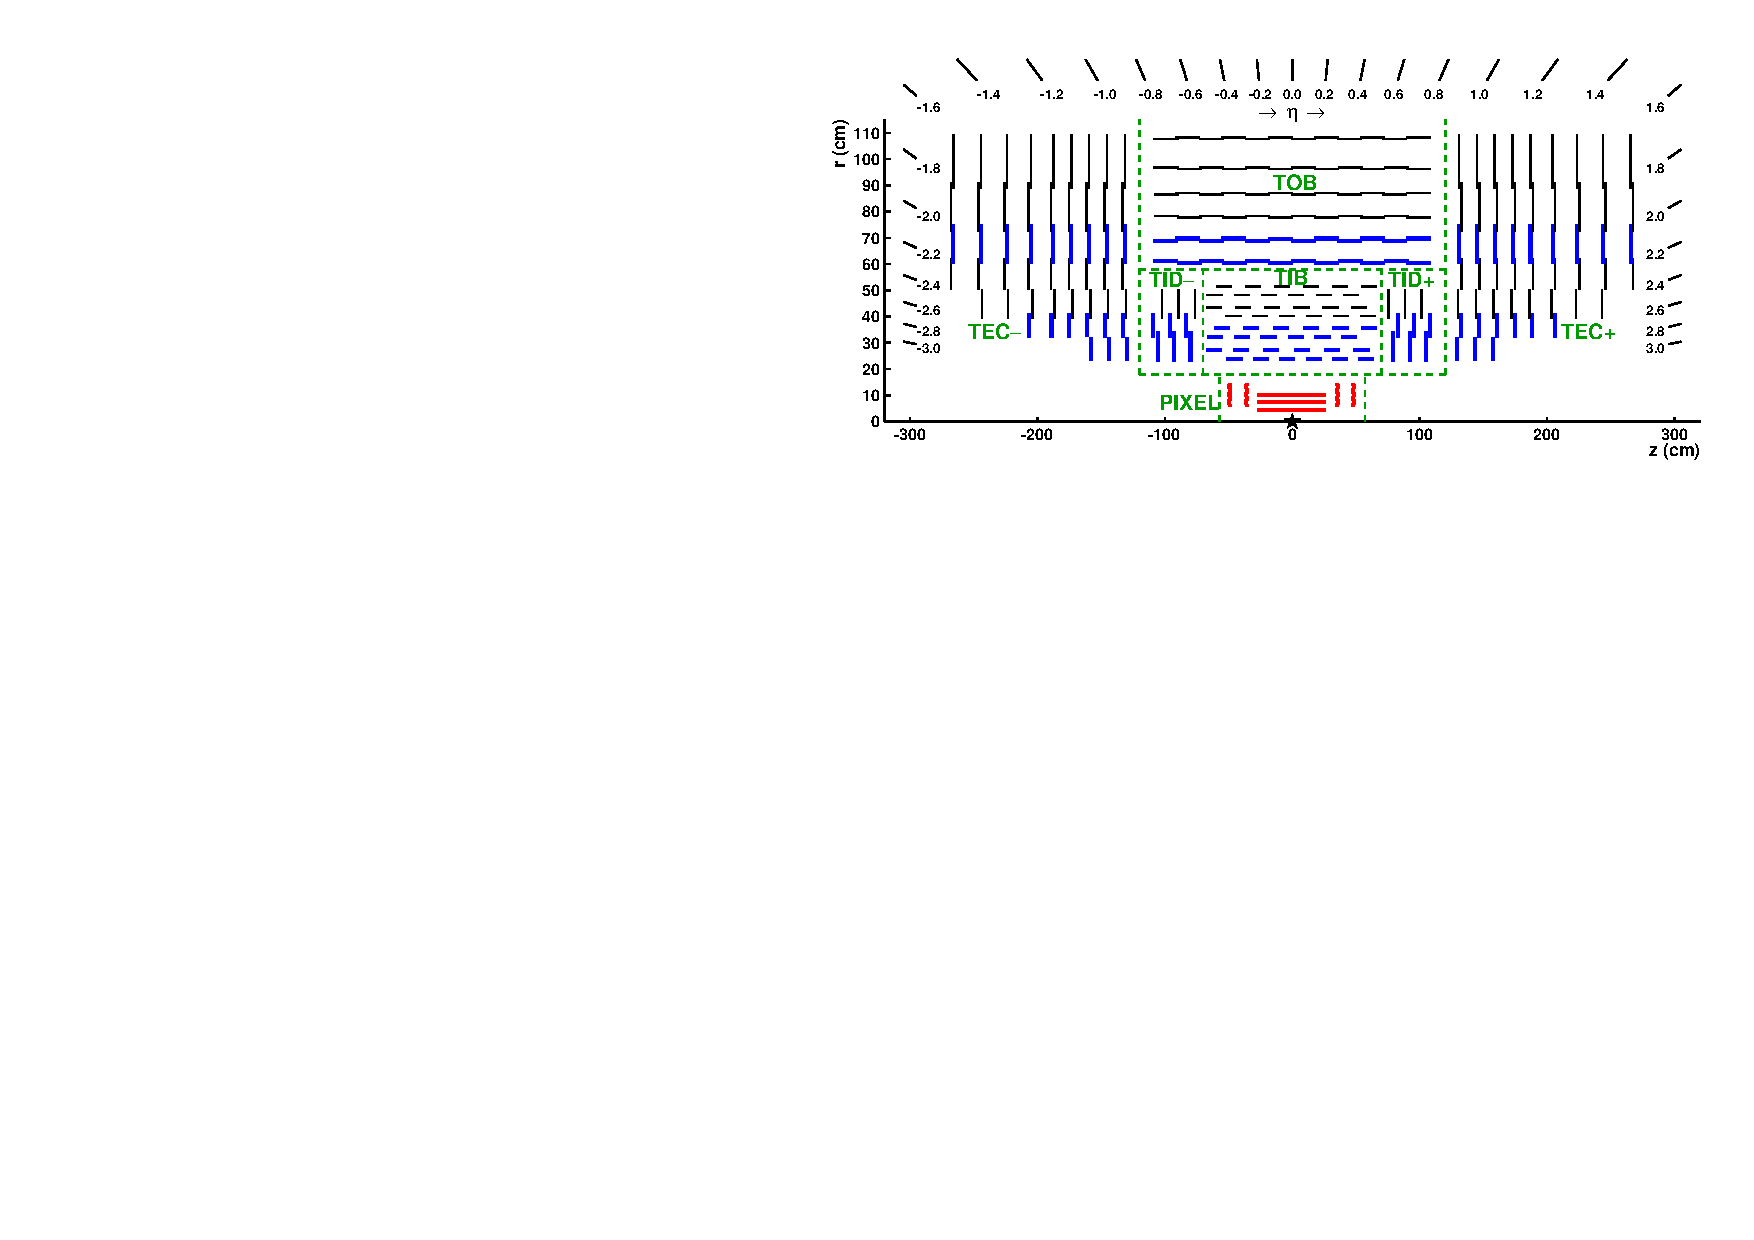
\includegraphics[width=12cm]{sst1}
  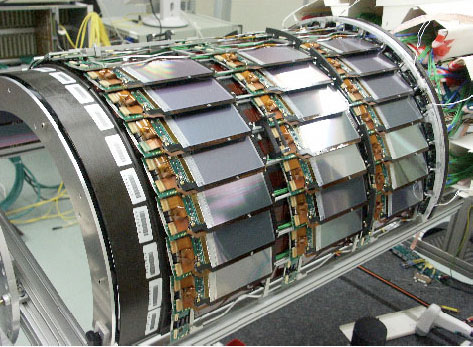
\includegraphics[width=6cm,height=4cm]{tib}
  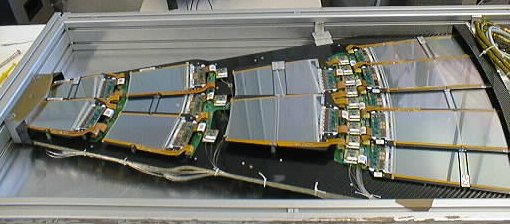
\includegraphics[width=6cm,height=4cm]{tec}
  %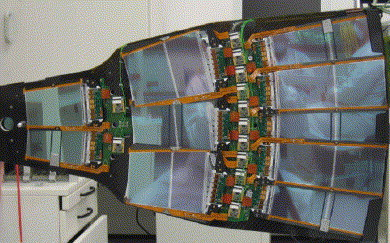
\includegraphics[width=6cm]{tec2}
  \caption[SST Schematic view.]{Top: CMS Siicon Strip Tracker (SST) schematic view. The SST is composed of the tracker inner barrel (TIB), the tracker inner disks (TID), the tracker outer barrel (TOB) and the tracker endcaps (TEC). Each part is made of silicon strip modules; the modules in blue represent two modules mounted back-to-back and rotated in the plane of the module by a stereo angle of 120 mrad in order to provide a 3-D reconstruction of the hit positions. Bottom: pictures of the TIB (left) and TEC (right) modules \cite{sst,tib,tec}.}
  \label{fig:sst}
\end{figure}

\noindent The silicon strip tracker (SST) is the second stage in the CMS tracking system . The top side of figure \ref{fig:sst} shows a schematic of the SST. The inner tracker region is composed of the tracker inner barrel (TIB) and the tracker inner disks (TID) covering the region $r<55$ cm and $|z|<118$ cm. The TIB is composed of 4 layers while the TID is composed of 3 disks at each end. The silicon sensors in the inner tracker are 320 $\mu$m thick, providing a resolution of about 13-38 $\mu$m in the $r\phi$ position measurement. \\

\noindent The modules indicated in blue in the schematic view of figure \ref{fig:sst} are two modules mounted back-to-back and rotated in the plane of the module by a ``stereo'' angle of 100 mrad; the hits from these two modules, known as ``stereo hits'', are combined to provide a measurement of the second coordinate (z in the barrel and r on the disks) allowing the reconstruction of hit positions in 3-D.\\ 

\noindent The outer tracker region is composed of the tracker outer barrel (TOB) and the tracker endcaps (TEC). The 6 layers of the TOB offers coverage in the region $r>55$ cm and $|z|<118$ cm, while the 9 disks of the TEC cover the region $124<|z|<282$ cm. The resolution offered by the outer tracker is about 13-38 $\mu$m in the $r\phi$ position measurement. The inner four TEC disks use silicon sensors 320 $\mu$m thick; those in the TOB and the outer three TEC disks use silicon sensors of 500 $\mu$m thickness. The silicon strips run parallel to the $z$-axis and the distance between strips varies from 80 $\mu$m in the inner TIB layers to 183 $\mu$m in the inner TOB layers; in the endcaps the wedge-shaped sensors with radial strips, whose pitch range between 81 $\mu$m at small radii and 205 $\mu$m at large radii.\\ 

\noindent The whole SST has 15148 silicon modules, 9.3 million silicon strips and cover a total active area of about 198 m$^2$ 

\subsection{Electromagnetic calorimeter}
\begin{figure}[h!]
  \centering
  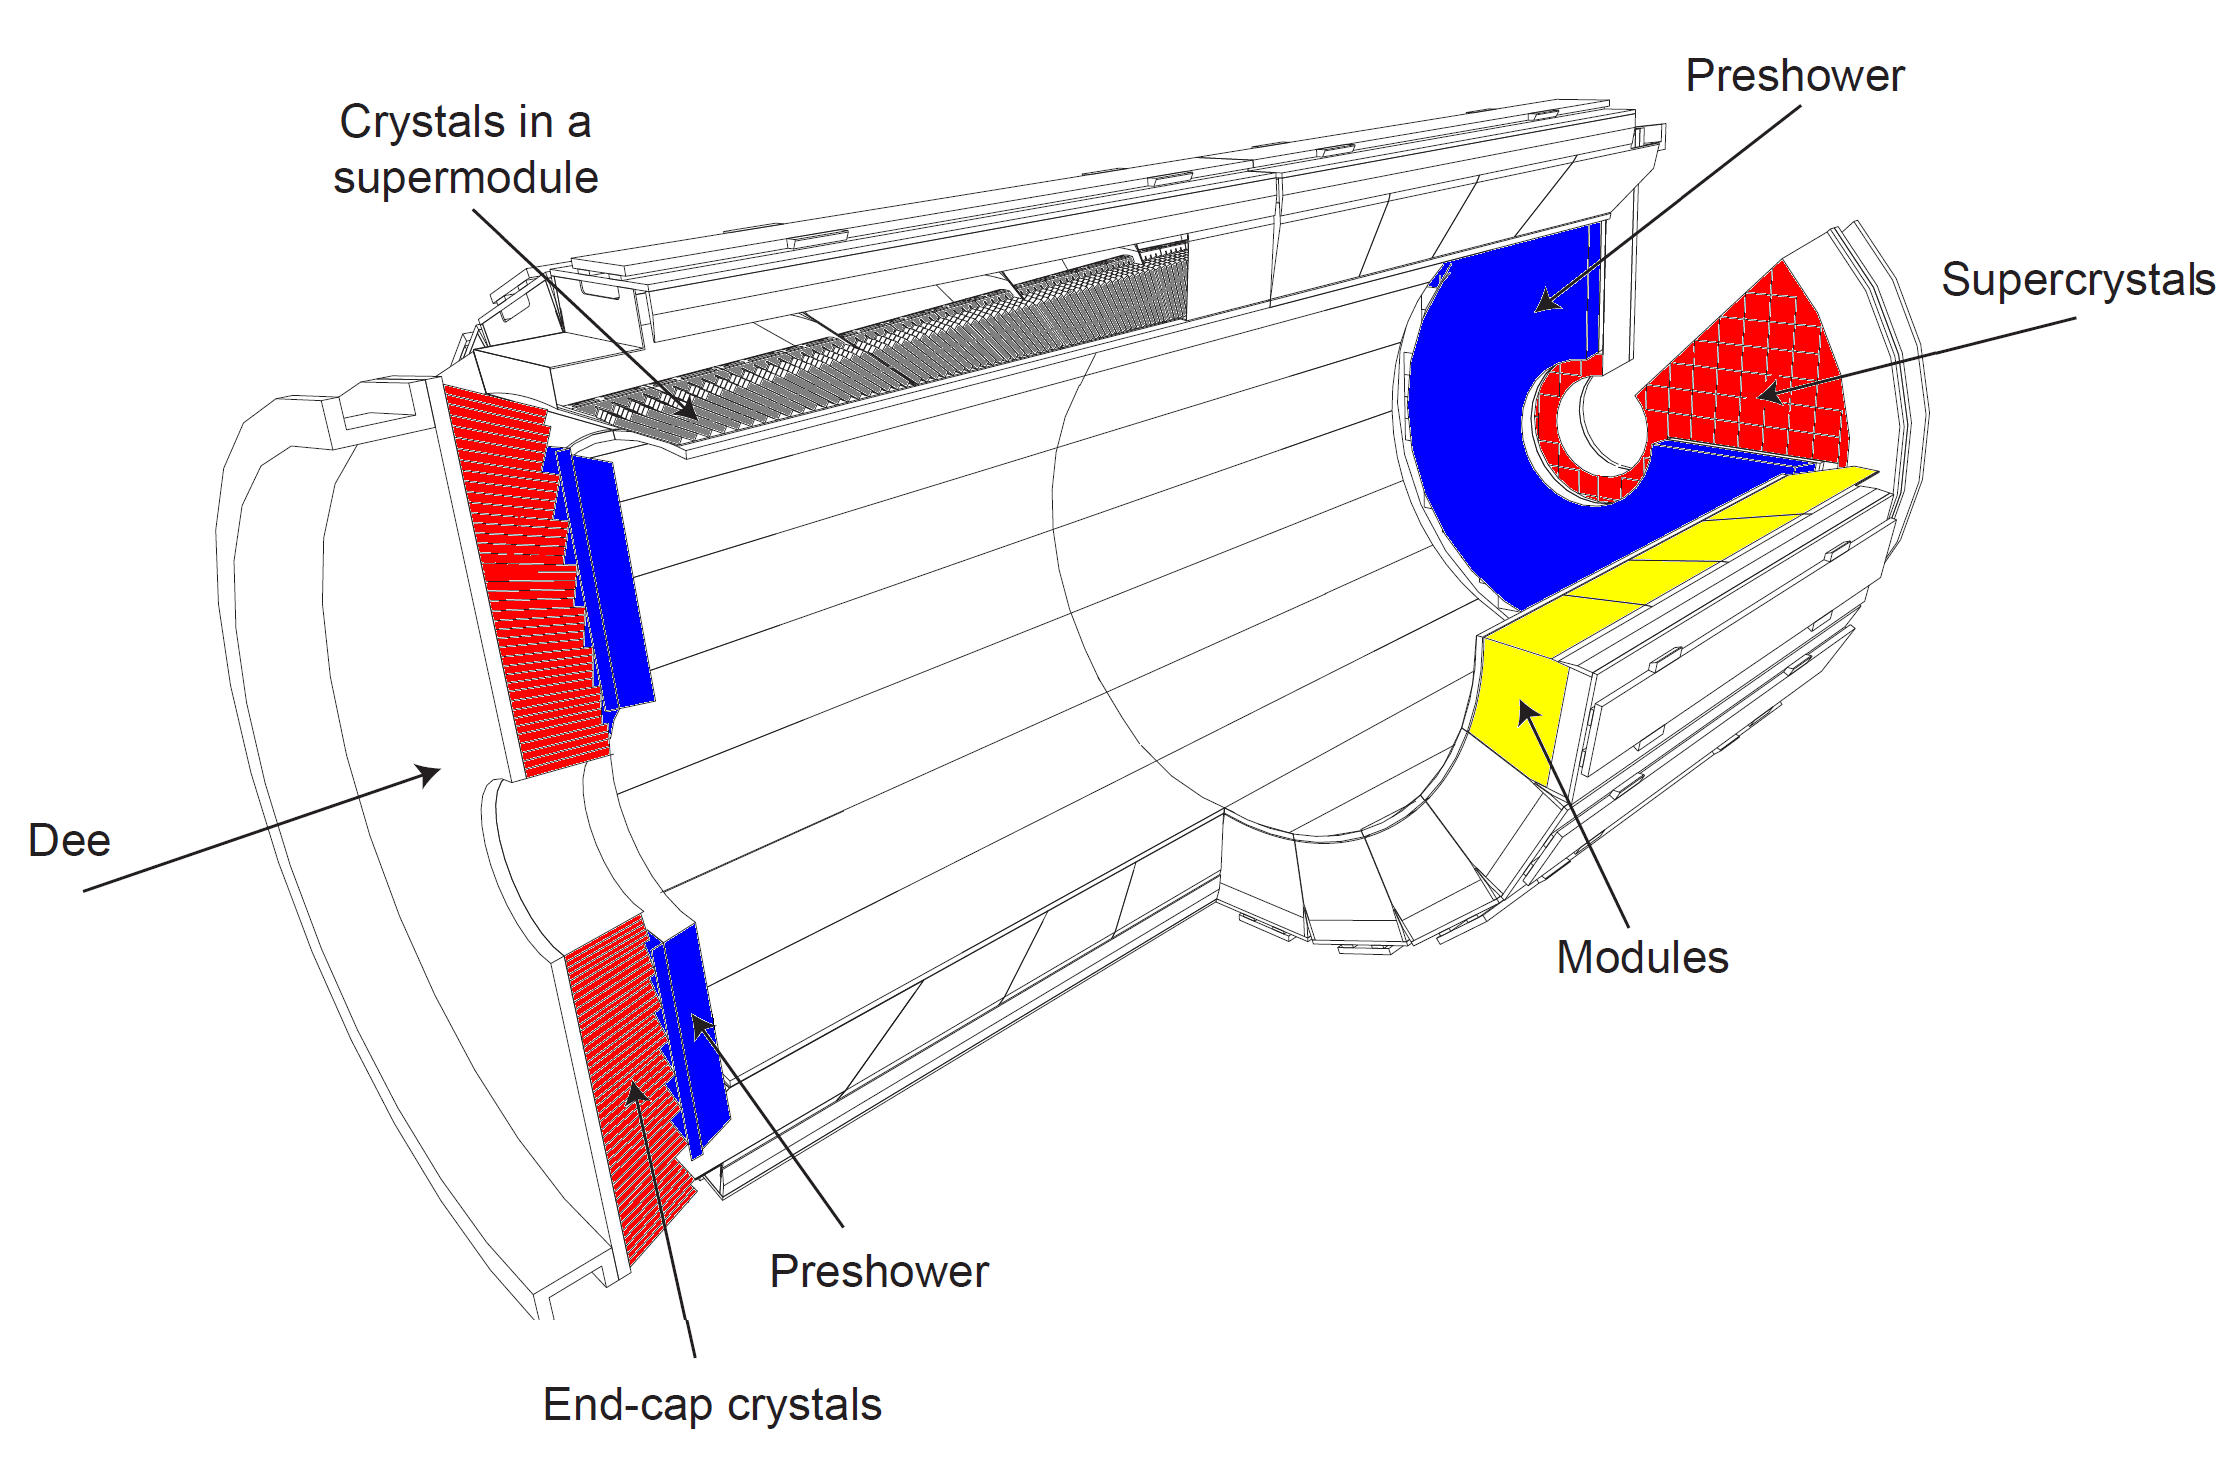
\includegraphics[scale=0.2]{ecal}
  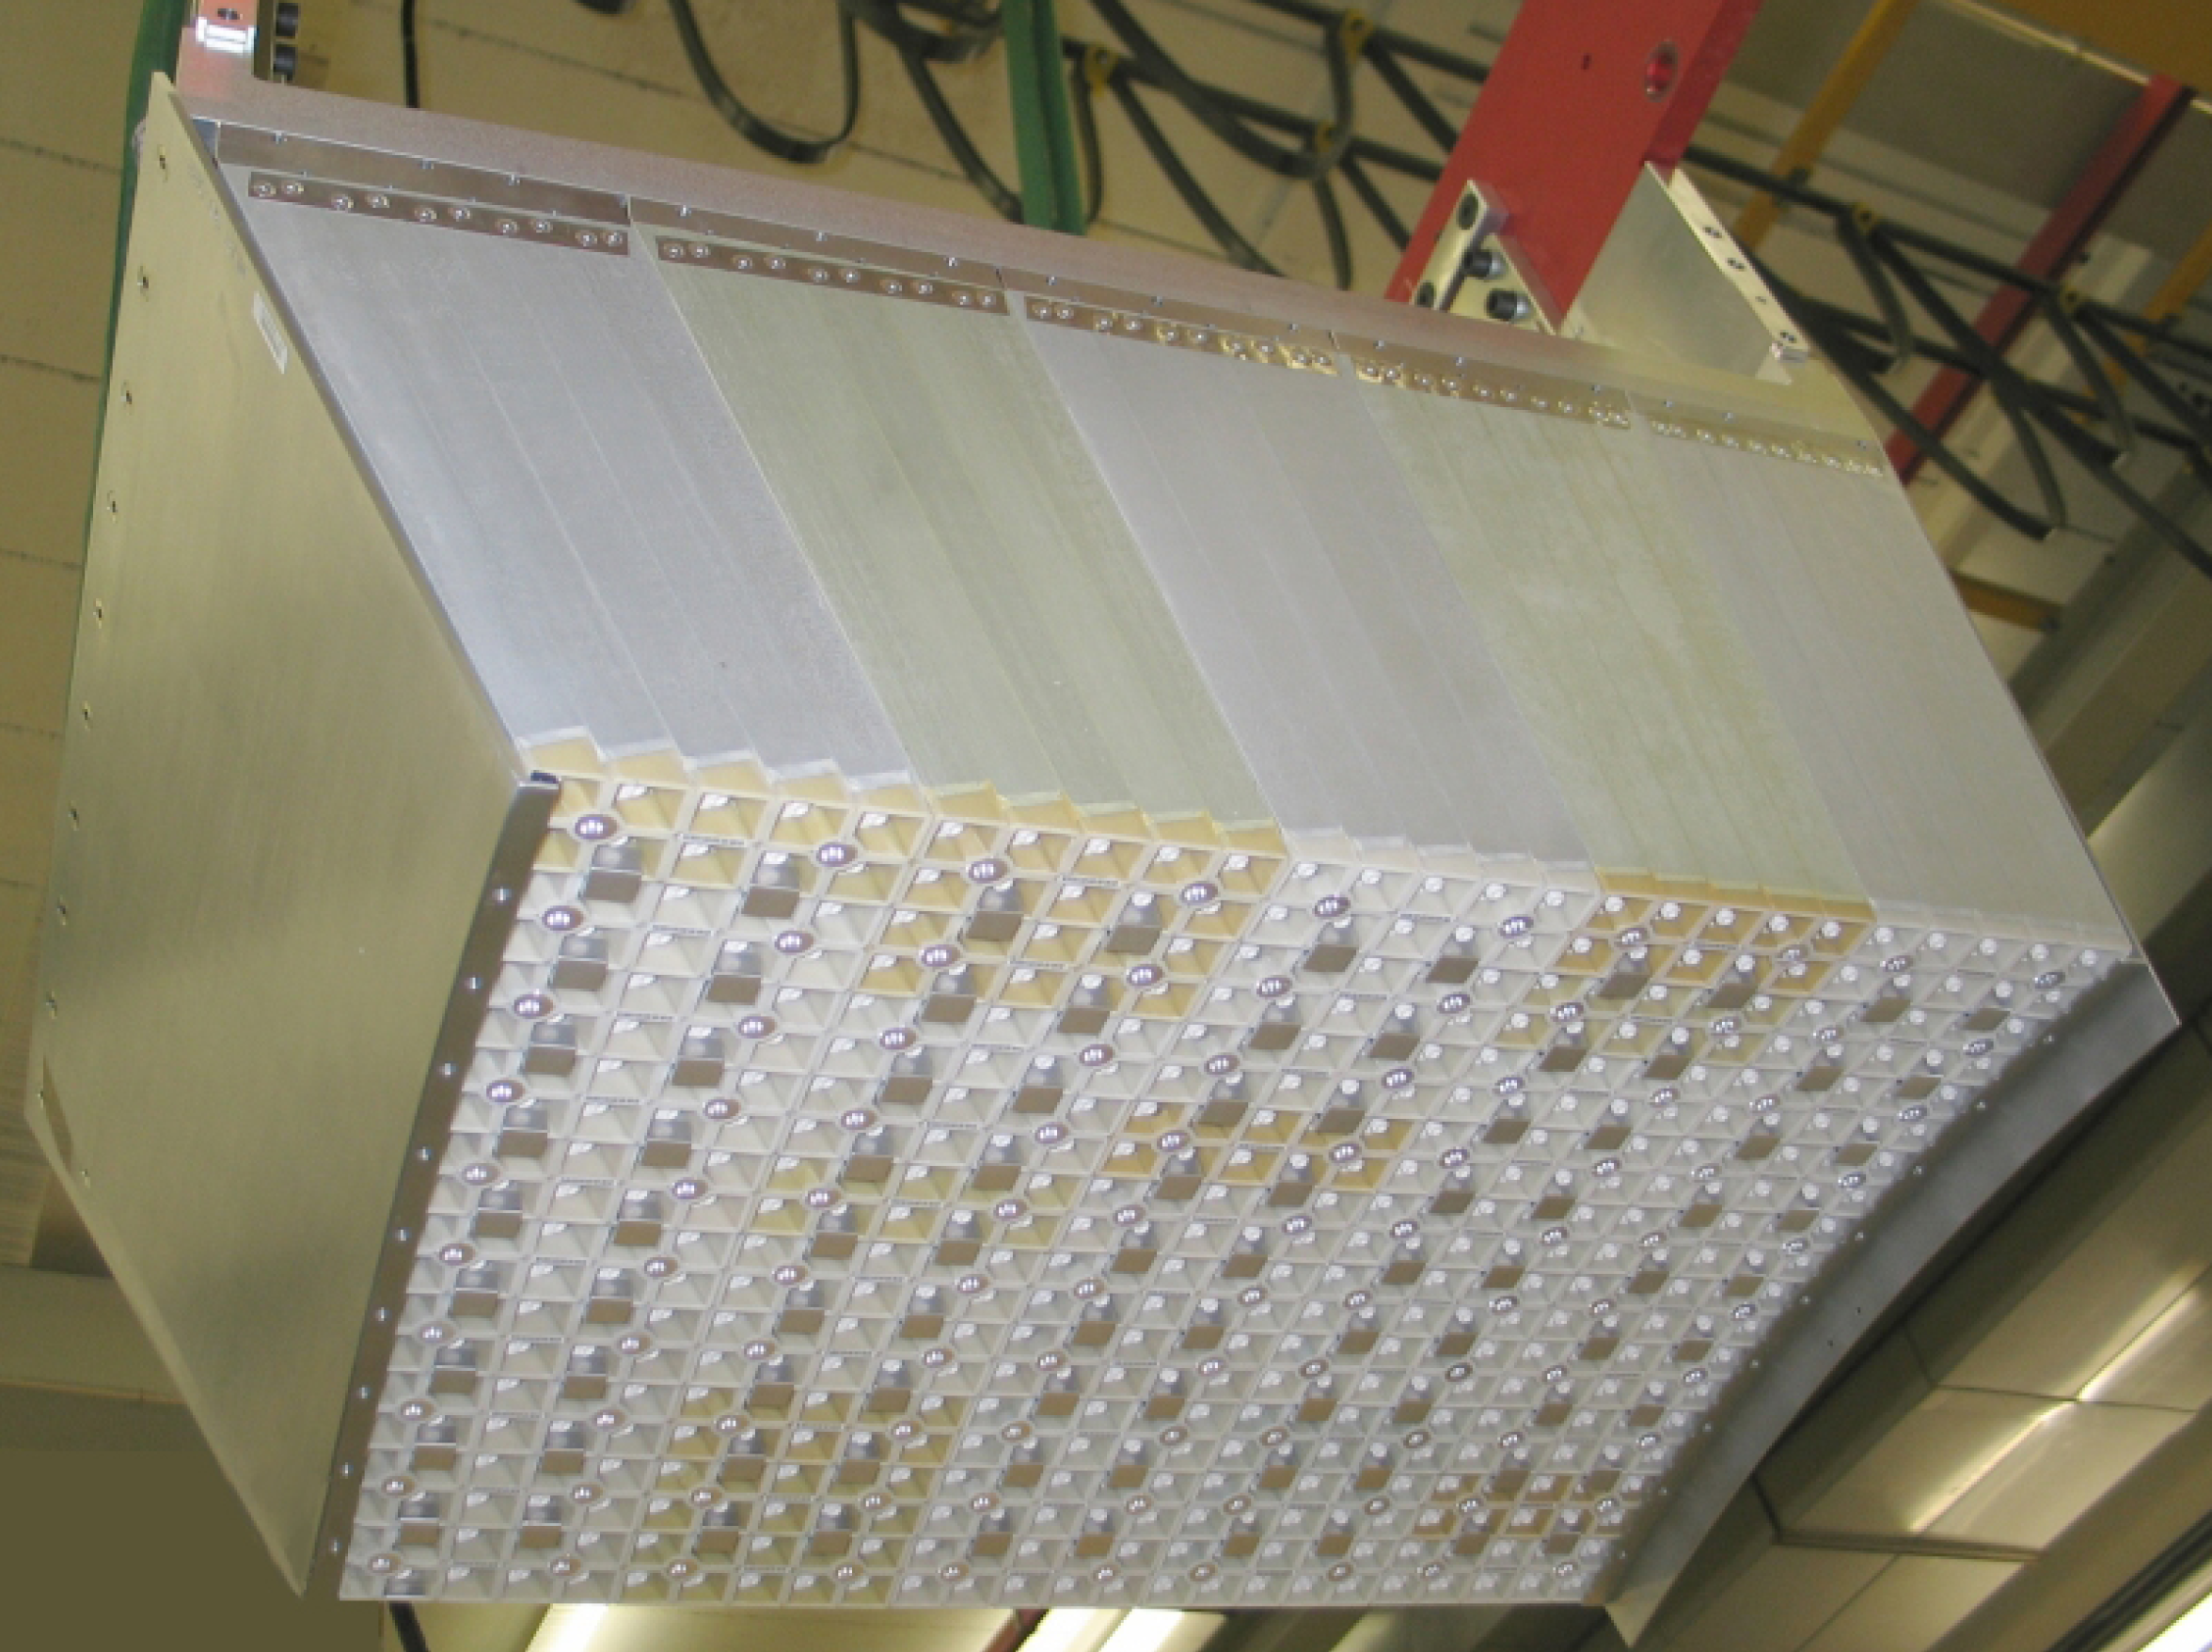
\includegraphics[width=6cm,height=4cm]{ecal_module}
  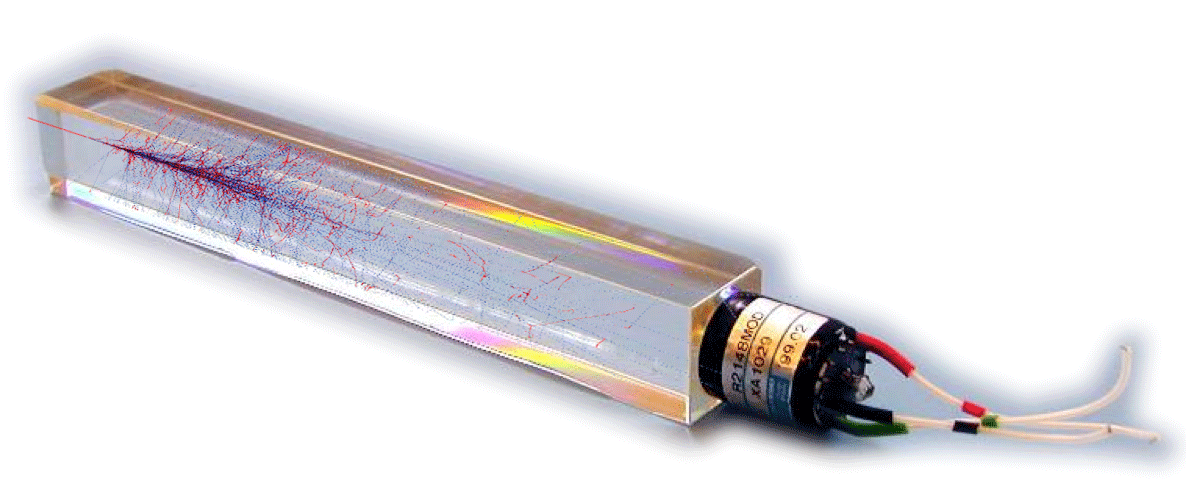
\includegraphics[width=6cm,height=4cm]{ecal_crystal} 
  \caption[CMS ECAL schematic view]{Top: CMS ECAL schematic view. Bottom: Module equipped with the crystals (left); ECAL crytal(right).}
  \label{fig:ecal}
\end{figure}

\noindent The CMS electromagnetic calorimeter (ECAL) is designed to measure the energy of electrons and photons. It is composed of 75848 lead tungstate crystals which has a short radiation length (0.89 cm) and fast response given that 80\% of the light is emmited within 25 ns; however, they are combined with Avalanche photodiodes (APDs) as photodetectors given that crytals themself have a low light yield (30$\gamma$/MeV). An schematic view of the ECAL is shown in figure \ref{fig:ecal}.\\

\noindent Energy is measured by absorbing electrons and photons which generates an electromagnetic ``shower'', as seen in bottom right picture of the figure\ref{fig:ecal}. The ECAL barrel (EB) cover the region $|\eta|$ < 1.479, using crystals of depth of 23 cm and  $2.2\times 2.2$ cm$^2$ transverse section. 

\noindent The ECAL endcap (EE) cover the region 1.479 < $|\eta|$ < 3.0 using crystals of depth 22 cm and transverse section of $2.86\times2.86$ cm$^2$; the photodetectors used are vacuum phototriodes (VPTs). Each EE is divided in two structures called ``Dees''.\\

\noindent In front of the EE, it is installed the preshower detector (ES) which covers the region $1.653 < |\eta| < 2.6$. The ES provides a precise measurement of the position of electromagnetic showers, which allows to distinguish electrons and photons signals from $\pi^0$ decay signals. The ES is composed of a layer of lead absorber followed by a layer of plastic scintillators

\subsection{Hadronic calorimeter}

\begin{figure}[h!]
  \centering
  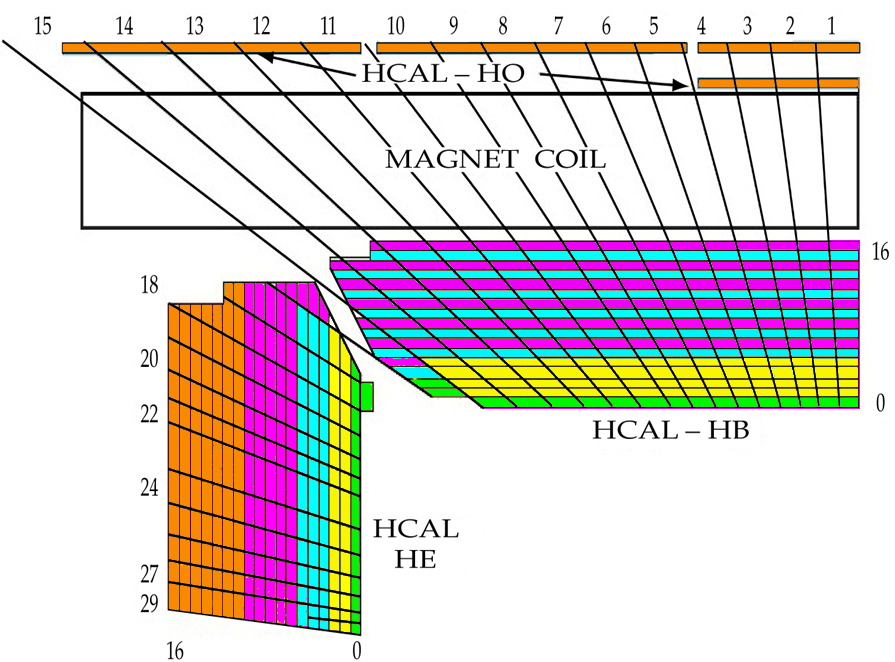
\includegraphics[scale=0.3]{hcal}\\
  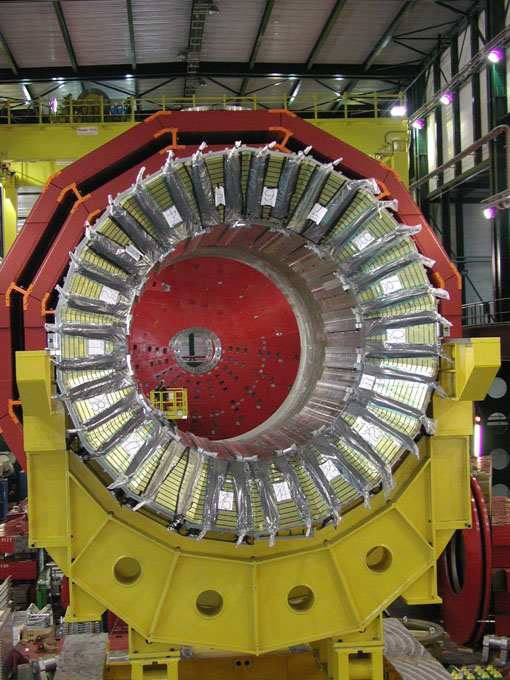
\includegraphics[width=3.5cm,height=4.5cm]{hb}
  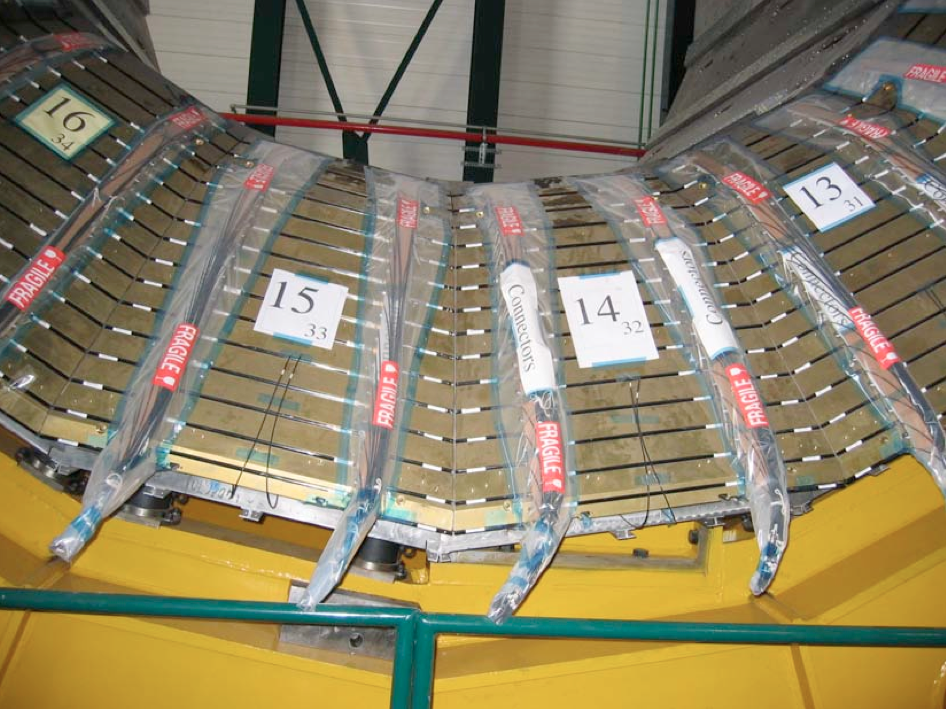
\includegraphics[width=4.5cm,height=4.5cm]{hb2}
  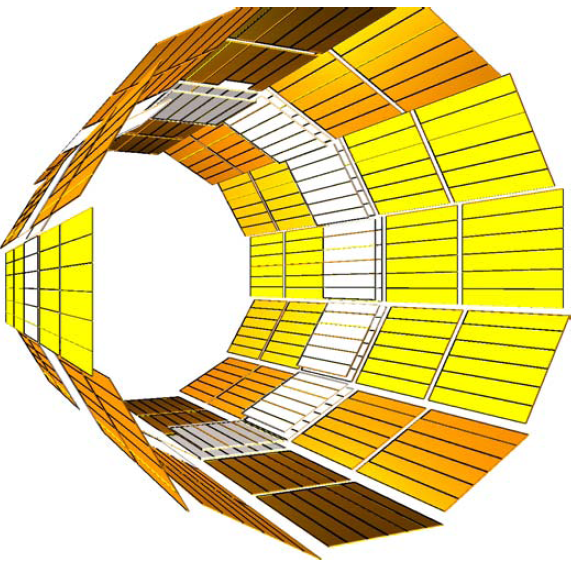
\includegraphics[width=4.5cm,height=4.5cm]{ho1} 
  \caption[CMS HCAL schematic view]{Top: CMS HCAL schematic view, the colors indicate the layers that are grouped into the same readout channels. Bottom: picture of a section of the HB; the absorber material is the golden region and scintillators are placed in between the absorber material (left and center). Schematic view of the HO (right).\cite{hcal,hb} }
  \label{fig:hcal}
\end{figure}

\noindent Hadrons are not absorbed by the ECAL but by the hadron calorimeter (HCAL), which is made of a combination of alternating brass absorber and silicon photomultiplier(SiPM) layers; therefore, particles passing through the scintillator material produce showers, as in the ECAL, as a result of the inelastic scattering of the hadrons with the detector material. Since the particles are not absorbed in the scintillator, their energy is sampled; therefore the total energy is not measured but stimated, which reduce the resolution of the detector. Brass was choosen as the absorber material due to its short interaction lenght ($\lambda_I=16.42$cm) and its non-magnetivity. Figure \ref{fig:hcal} shows an schematic view of the CMS HCAL.\\

\noindent The HCAL is divided in four sections; the Hadron Barrel (HB), the Hadron Outer (HO), the Hadron Endcap (HE) and the Hadron Forward (HF) sections. The HB cover the region $0<|\eta|<1.4$, while the HE covers the region $1.3<|\eta|<3.0$. The HF, made of quartz fiber scintillator and steel as absorption material, covers the forward region $3.0<|\eta|<5.2$. Both the HB and HF are located inside the solenoid. The HO is placed outside the magnet as an additional layer of scintillators with the purpose of measure the energy tails of particles passing through the HB and the magnet (see figure \ref{fig:hcal} top and bottom right) . The upgrades made to the HCAL during the technical stop 2016-2017 consisted in the replacement of the phototransducers, improving the efficiency.

\subsection{Superconducting solenoid magnet}

\begin{figure}[h!]
  \centering
  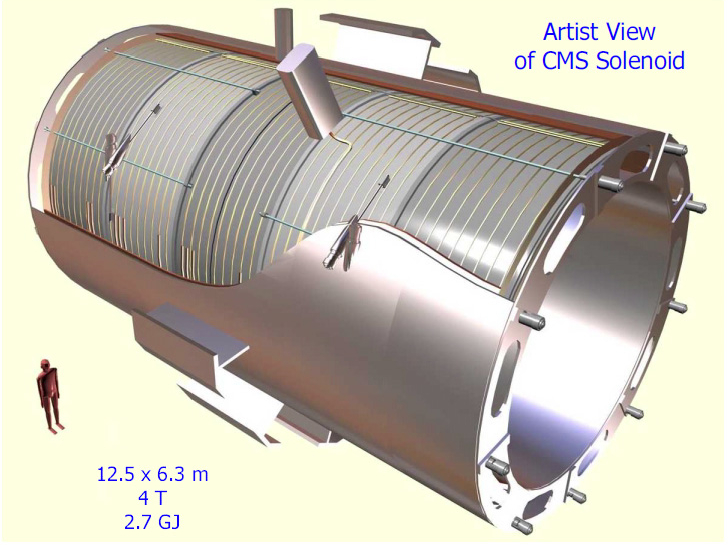
\includegraphics[scale=0.38]{magnet}
  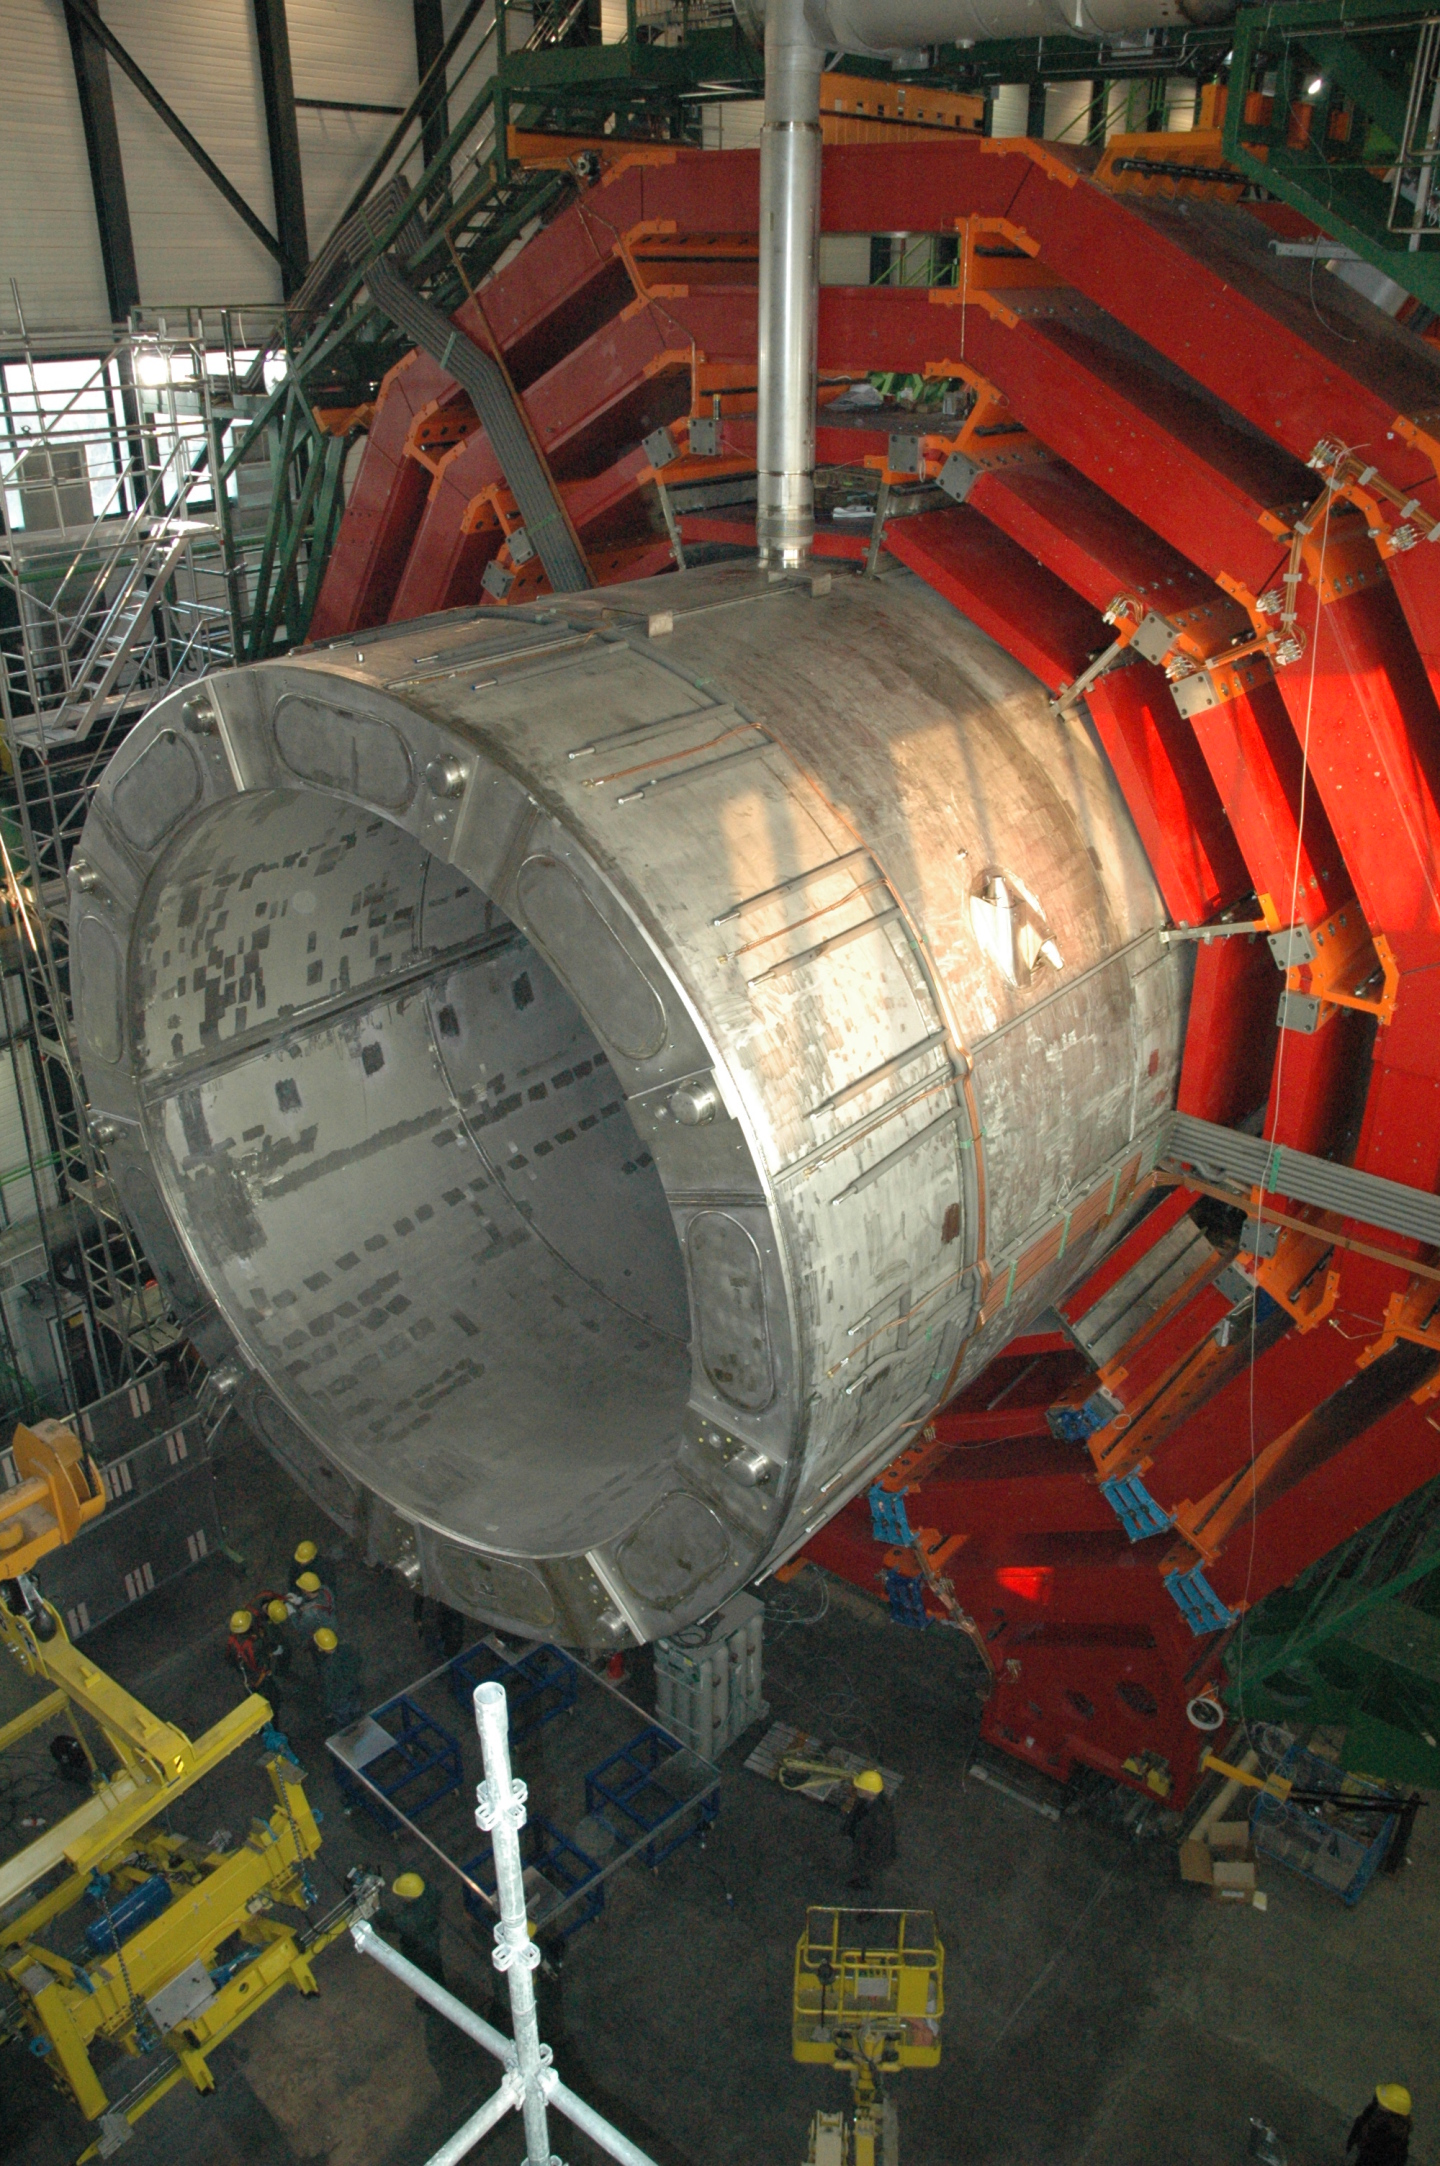
\includegraphics[scale=0.4]{yoke2}
  %\includegraphics[scale=0.4]{yoke1} 
  \caption[CMS solenoid magnet]{Artistic representation of the CMS solenoid magnet(left). The magnet is supported on an iron yoke (right) which also serves as the house of the muon detector and as mechanical support for the whole CMS detector \cite{yoke2}.}
  \label{fig:yoke}
\end{figure}

\noindent The superconducting magnet installed is the CMS detector is designed to provide an intense and highly uniform magnetic field in the central part of the detector. In fact, the tracking system takes advantage of the bending power of the magnetic field to measure with precision the momentum of the particles that traverse it; the unambiguous determination of the sign for high momentum muons was a driven principle  during the design of the magnet. The magnet has a diameter of 6.3 m, a length of 12.5 m in a cold mass of 220 t; the generated magnetic field reach a strength of 3.8T. Since it is made of Ni-Tb superconducting cable it has to operate at a temperature of 4.7 K by using a helium cryogenic system; the current circulating in the cables reach 18800 A under normal running conditions. The left side of figure \ref{fig:yoke} shows an artistic view of the CMS magnet, while the right side shows a transverse view of the cold mass where the winding structure is visible. \\

\noindent The yoke (see figure \ref{fig:yoke}), composed of 5 barrel wheels and 6 endcap disks made of iron, serves not only as the media for magnetic flux return, but also provides the house for the muon detector sytem and structural stability to the full detector.     

\subsection{Muon system }

\begin{figure}[h!]
  \centering
  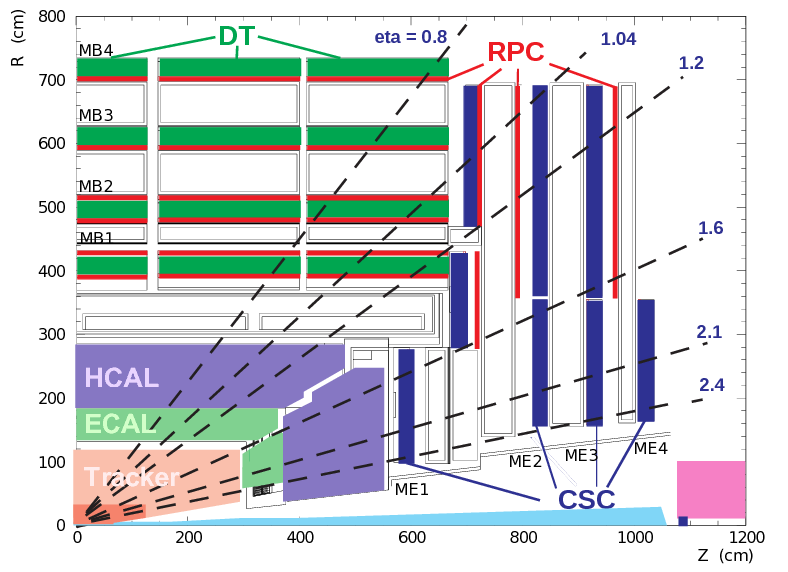
\includegraphics[width=10cm,height=6cm]{muon}
  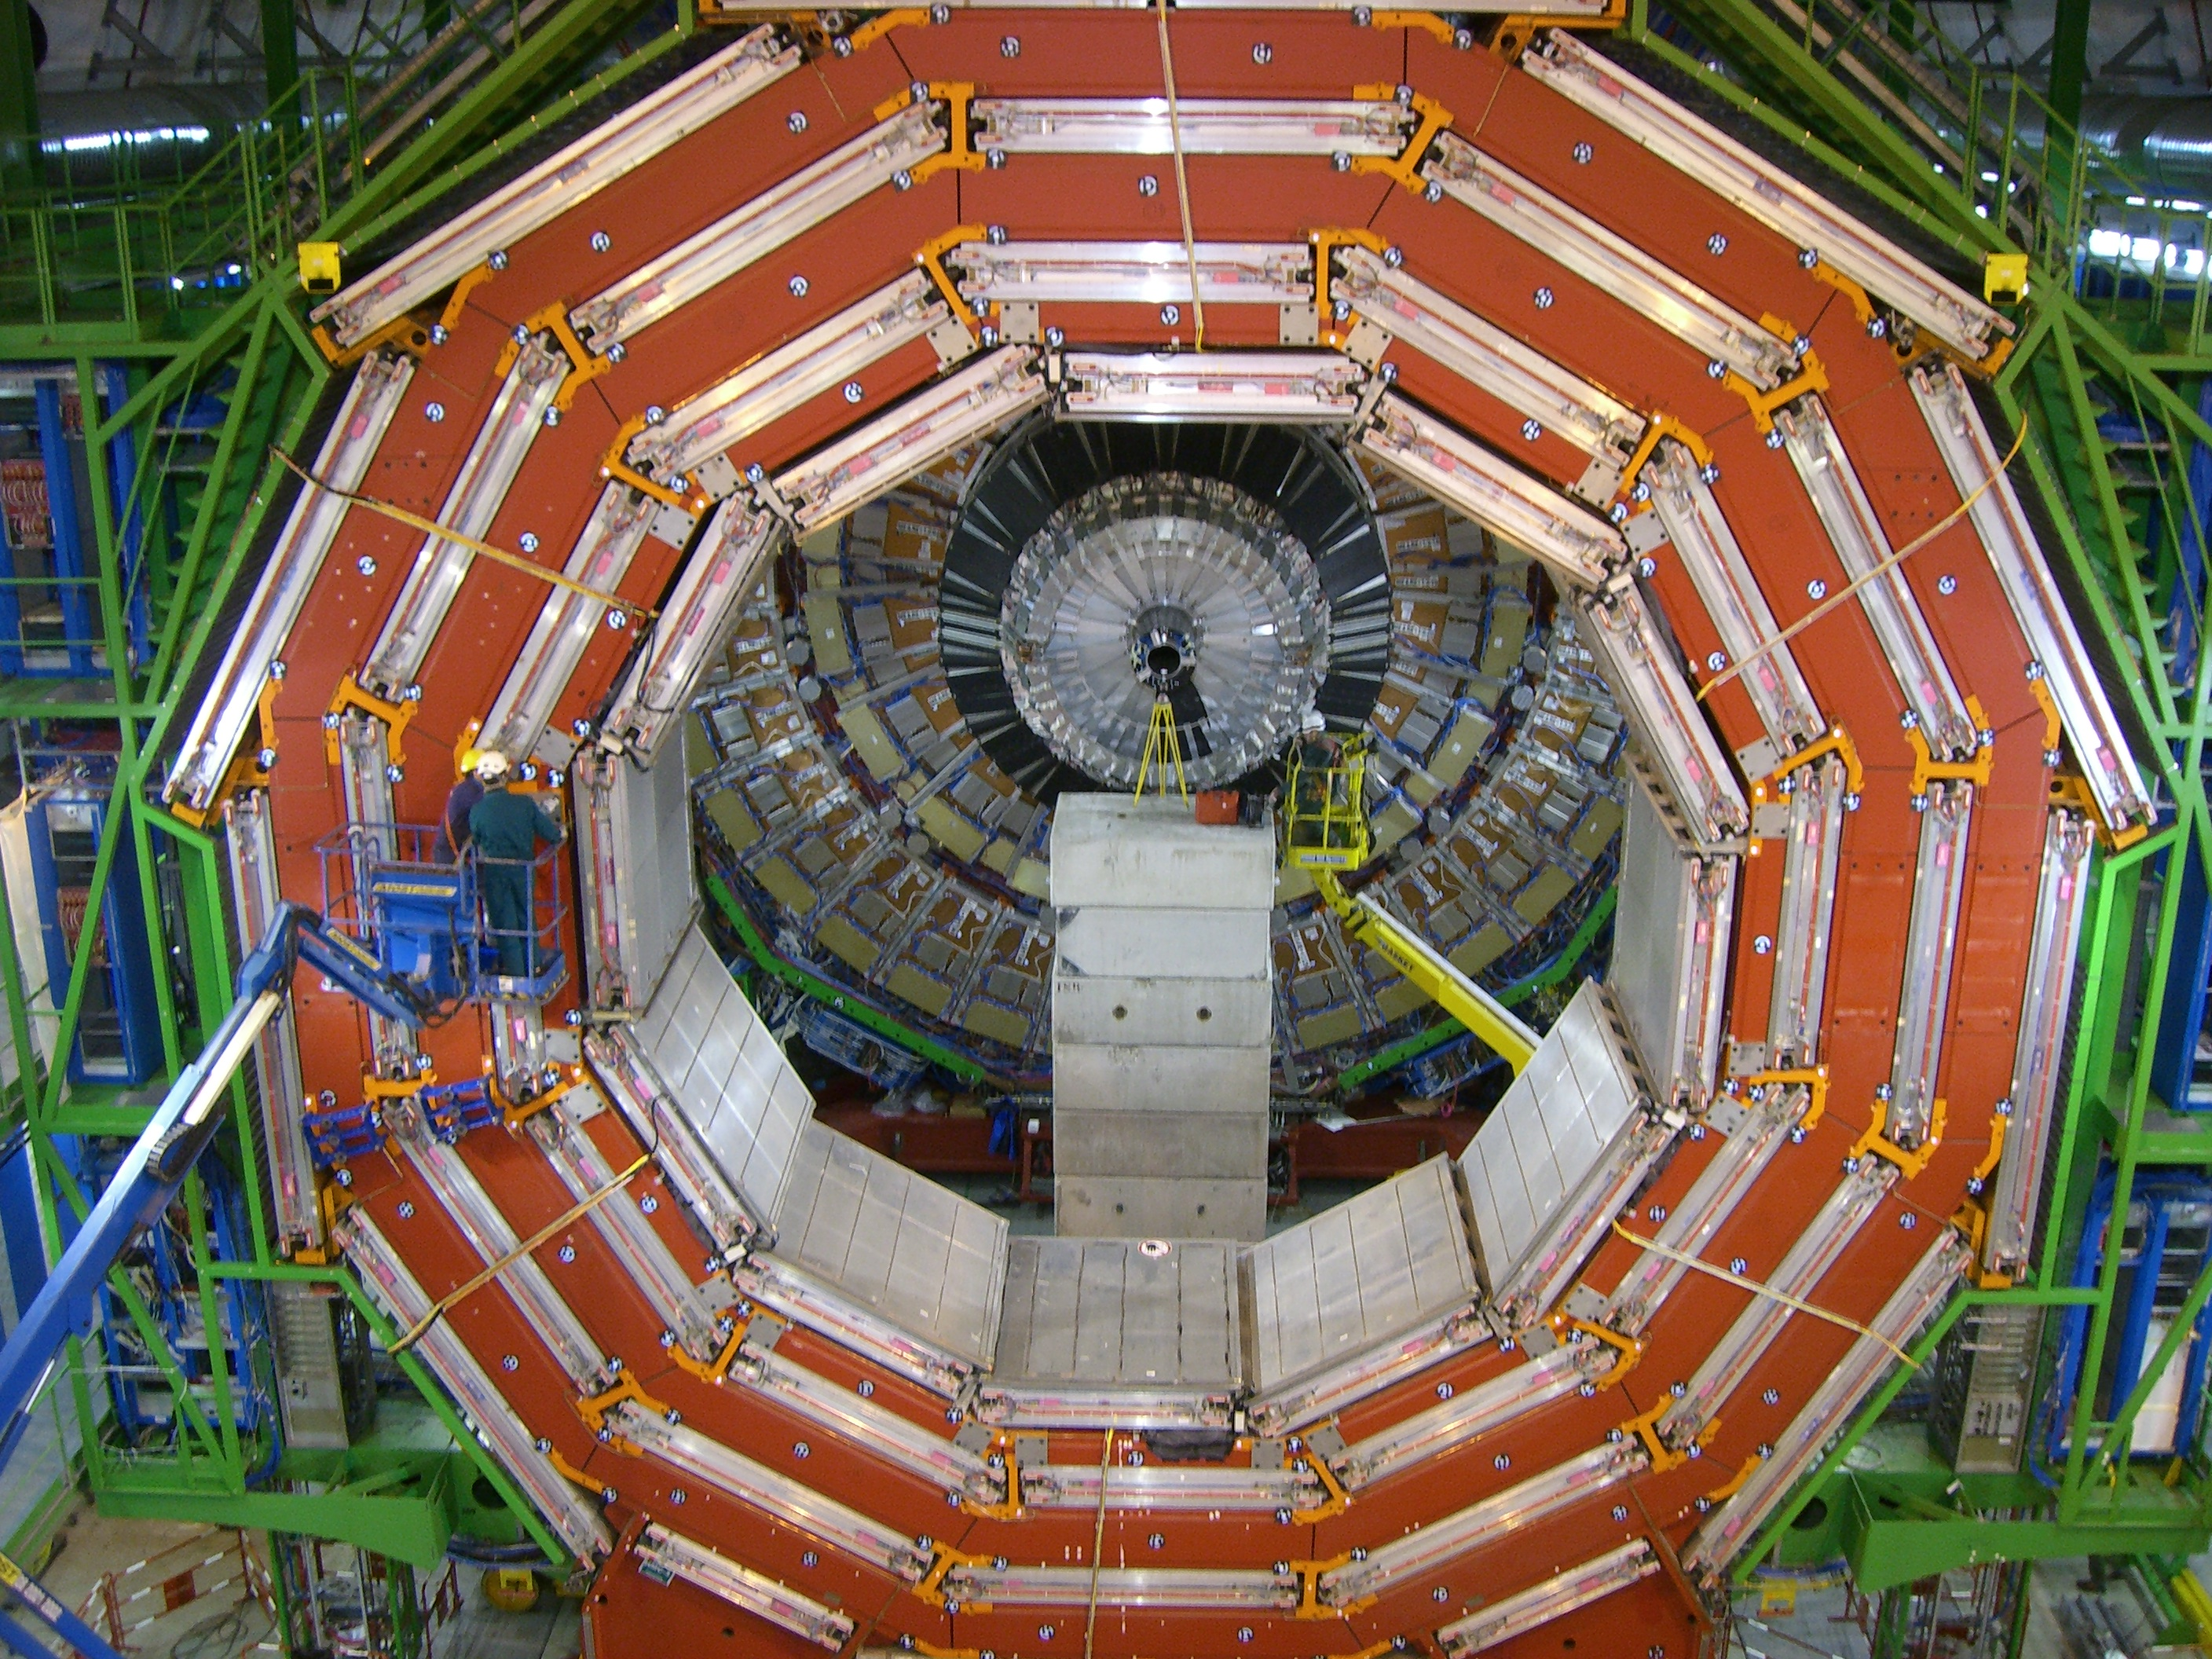
\includegraphics[width=5cm,height=4.55cm]{muon2}
  \caption[CMS Muon system schematic view]{Left: CMS muon system schematic view; Right: one of the yoke rings with the muon DTs and RPCs installed; in the back it is posible to see the muon endcap\cite{muon}. }
  \label{fig:muon_chambers}
\end{figure}

\noindent Muons are the only charged particles able pass through all the CMS detector due to their low ionization energy loss; thus, muons can be separated easily from the high amount of particles produced in a pp collision. Also, muons are expected to be produced in the decay of several new particles; therefore, a good detection of muons was on the leading principles when designing the CMS detector.\\

\noindent The CMS muon detection system is embedded in the return yoke as seen in figure \ref{fig:muon_chambers}. It is composed of three different detector types; the drift tube chambers (DT) are located in the central region $\eta< 1.2$ arranged in four layers of drift chambers filled with an Ar/CO$_2$ gas mixture.\\

\noindent The muon endcaps are made of Cathode strip chambers (CSC) covering the region $\eta< 2.4$ and filled with a mixture of Ar/CO$_2$/CF$_4$. The reason behind using a different detector type lies on the different conditions in the forward region like the high muon rate and high residual magnetic field.\\

\noindent The third type of detector used in the muon system is a set four disks of resistive plate chambers (RPC) working in avalanche mode. The RPCs provide good spatial and time resolutions. The track of $high-p_T$ muon candidate is build combining information from the tracking system and the signal from up to 6 RPCs and 4 DT chambers.
\subsection{trigger system - HLT- L1 }


The
online event selection process (trigger) must reduce the huge rate to about 100 events/s for storage
and subsequent analysis. The short time between bunch crossings, 25 ns, has major implications
for the design of the read-out and trigger systems.


Due to its high segmentation, the pixel detector not only forms high quality seeds for
the track reconstruction algorithm offline, but is also used to do fast tracking online in the high
level trigger (HLT) for primary vertex reconstruction, electron/photon identification, muon
reconstruction, tau identification and b-tagging.



\subsection{ computing model}
\section{Event generation  simulation and reconstruction}
\subsection{ event generation}
\subsection{Hard scattering  }
\subsection{parton shower }
\subsection{hadronization and decays }
\subsection{underlying events and pileup }
\subsection{ MC - MadEvent, MadGraph and madgraph\@NLO, powheg, pythia, tauola}
\subsection{ detector simulation}
\subsection{event reconstruction- particle flow algorithm, vertexing , muon reco, electron reco, photon and hadron reco, jets reco, anti-kt algoritm, jet energy corrections, btagging, MET  }
\subsection{ MVA methods, NN, BDT, boosting, overtraining, variable ranking  }
\subsection{statistical inference, likelihood parametrization}
\subsection{ nuisance paraeters}
\subsection{exclusion limits }
\subsection{asymptotic limits }

